\pdfminorversion=4
\documentclass[xcolor={usenames,dvipsnames,svgnames,table}]{beamer}
%for printing or having a crappy pdf reader backup
%\documentclass[handout]{beamer}
\mode<presentation>
\usetheme{Madrid}

% this file contains all commonly used packages for the Rattlesnake documentation
% new package, add comment what they are used for

% command packages
\usepackage{xifthen}     % if -then else command

% language and font improvements
\usepackage[english]{babel}	% Multilingual support - https://www.ctan.org/pkg/babel
\usepackage[utf8]{inputenc} % Accept different input encodings - https://www.ctan.org/pkg/inputenc
\usepackage[kerning,spacing,babel]{microtype} % Subliminal refinements towards typographical perfection - https://www.ctan.org/pkg/microtype
\usepackage{eepic}      % Extensions to epic - https://www.ctan.org/pkg/eepic
\usepackage{epic}       % Enhance LaTeX picture mode - https://www.ctan.org/pkg/epic
\usepackage[T1]{fontenc} % selecting font encodingsselecting font encodings - https://www.ctan.org/pkg/fontenc
\usepackage{lmodern}

% title packages
\usepackage{authblk}		% footnote style author/affiliation - https://www.ctan.org/pkg/authblk

% symbols
\usepackage{upgreek}		% Upright Greek letters - https://www.ctan.org/pkg/upgreek
\usepackage{cancel}			% \cancel cmd - https://www.ctan.org/pkg/cancel

% chemical and isotope packages
\usepackage{isotope}		% isotope command - https://www.ctan.org/pkg/isotope
\usepackage{mhchem}			% chemical formulae/equations - https://www.ctan.org/pkg/mhchem

% layout packages
\usepackage{xspace}			% smart space \xspace - https://www.ctan.org/pkg/xspace
\usepackage{icomma}			% smart math comma - https://www.ctan.org/pkg/icomma
\usepackage{chngpage}		% page layout change during document - https://www.ctan.org/pkg/chngpage
\usepackage[usenames,dvipsnames,svgnames,table]{xcolor}			% color definitions - https://www.ctan.org/pkg/xcolor
\usepackage{enumitem}   % layout for itemize and enumerate - http://www.ctan.org/pkg/enumitem
\usepackage{setspace}    % allows for \singlespacing, \onehalfspacing, and \doublespacing commands - https://www.ctan.org/pkg/setspace

% floating packages
% needed by the breakalgo environment labelsep=quad
\usepackage[singlelinecheck=false, labelsep=quad]{caption}	% table captions - https://www.ctan.org/pkg/caption
\usepackage{subcaption}		% Support for sub-captions - https://www.ctan.org/pkg/subcaption
\usepackage{placeins}   	% Control float placement - https://www.ctan.org/pkg/placeins
\usepackage{float}      	% Improved interface for floating objects - https://www.ctan.org/pkg/float

% table packages
\usepackage{supertabular}	% multi-page tables package - https://www.ctan.org/pkg/supertabular
\usepackage{booktabs}		% table settings - https://www.ctan.org/pkg/booktabs
\usepackage{array}			% Extending the array and tabular environments - https://www.ctan.org/pkg/array
\usepackage{multirow}		% tabular cells spanning multiple rows - https://www.ctan.org/pkg/multirow
% \usepackage{tabls}      % Better vertical spacing in tables and arrays - https://www.ctan.org/pkg/tabls
\usepackage{colortbl}      % Allows for color manipulation within tables - https://www.ctan.org/pkg/colortbl

% pictures, plots and listings
\usepackage{graphicx}		% include graphics - https://www.ctan.org/pkg/graphicx
\usepackage{wrapfig}		% wrapfigure enviroment - https://www.ctan.org/pkg/wrapfig
\usepackage{pgfplots}		% latex plots - https://www.ctan.org/pkg/pgfplots


% source code and algorithms
\usepackage{algorithmicx} % newer version of algorithmic - https://www.ctan.org/pkg/algorithmicx
\usepackage{listings} 	% source code listings - http://www.ctan.org/pkg/listings
\usepackage{verbatim}   % verbatim - https://www.ctan.org/pkg/verbatim

% misc packages
\usepackage{url}        % provide \url command for web addresses - https://www.ctan.org/pkg/url
\usepackage{import}			% Establish input relative to a directory - https://www.ctan.org/pkg/import
\usepackage{afterpage}  % Execute command after the next page break - https://www.ctan.org/pkg/afterpage
\usepackage{lscape}     % Place selected parts of a document in landscape - https://www.ctan.org/pkg/lscape
\usepackage{rotating}   % Rotation tools, including rotated full-page floats - https://www.ctan.org/pkg/rotating
\usepackage{chngcntr}   % Change the resetting of counters - http://ctan.org/pkg/chngcntr
\usepackage{textpos}    % Allows logo and banner manipulation

% eps support
\usepackage{epsfig}       % include eps figures - https://www.ctan.org/pkg/epsfig
\usepackage{epsf}          % Simple macros for EPS inclusion - https://www.ctan.org/pkg/epsf
\usepackage{epstopdf}   %use .eps images (as pdf) in \includegraphics


% reference packages
% hyperref must be loaded before amsmath to avoid problems with subequations and align
\usepackage{hyperref}		% Extensive support for hypertext - https://www.ctan.org/pkg/hyperref


% packages that must be loaded after hyperref - http://tex.stackexchange.com/questions/1863/which-packages-should-be-loaded-after-hyperref-instead-of-before
\usepackage{geometry}		% Flexible and complete interface to document dimensions - https://www.ctan.org/pkg/geometry
\usepackage{algorithm}  % algorithm enviroment

% ams math packages
\usepackage{amsmath}    % mathematical facilities - https://www.ctan.org/pkg/amsmath
\usepackage{amsfonts}   % fonts for math - https://www.ctan.org/pkg/amsfonts
\usepackage{amssymb}    %
\usepackage{amsthm}     % Typesetting theorems - https://www.ctan.org/pkg/amsthm

\usepackage{nameref}		% allows references with names instread of numbers \nameref - http://www.ctan.org/pkg/nameref
\usepackage[capitalize,nameinlink]{cleveref}   % smart references - http://ctan.org/pkg/cleveref

\makeatletter
% prevent a package from loading
\newcommand{\dontusepackage}[2][]{%
    \@namedef{ver@#2.sty}{9999/12/31}%
    \@namedef{opt@#2.sty}{#1}
}

% a macro to load packages only if they are not yet loaded, needed for combination of beamer and hyperref
\newcommand{\usepackagesave}[2][{}]{
    \ltx@ifpackageloaded{#2}{}{
        \usepackage[#1]{#2}}
}
\makeatother
%Prevent authblk from loading
\dontusepackage{authblk}


\usecolortheme[RGB={128,128,128}]{structure}
\definecolor{my_gray}{RGB}{105,105,105}
\setbeamercolor{khumna}{fg=white,bg=my_gray}
%teal \usecolortheme[RGB={0,128,128}]{structure}
%\useoutertheme{miniframes}
\useinnertheme{default}
\definecolor{Maroon}{RGB}{80,0,0}
\definecolor{BurntOrange}{RGB}{204,85,0}

\usepackage[figurename=,tablename=]{caption}
\setbeamercolor{normal text}{fg=black}
\setbeamercovered{dynamic}
\beamertemplatetransparentcovereddynamicmedium
\setbeamertemplate{caption}[numbered]
\usepackage{colortbl}
\newcommand {\mathsym}[1]{{}}
\newcommand {\unicode}{{}}
\newcommand{\om}{\boldsymbol{\Omega}}
\newcommand{\etal}{{\it et al.\,}}
\newcommand{\vr}{\vec{r}}
\newcommand{\vo}{\vec{\Omega}}
\newcolumntype{L}{>{\centering\arraybackslash}m{3cm}}
\newcommand{\tcr}[1]{\textcolor{red}{#1}}
%Creating a norm command
\newcommand{\norm}[1]{\left\lVert#1\right\rVert}
%Allow page breaks within align
\allowdisplaybreaks



\newlength \figwidth
\setlength \figwidth {0.5\textwidth}

\newcommand{\backupbegin}{
   \newcounter{finalframe}
   \setcounter{finalframe}{\value{framenumber}}
}
\newcommand{\backupend}{
   \setcounter{framenumber}{\value{finalframe}}
}

\addtobeamertemplate{frametitle}{}
{
	\begin{textblock*}{100mm}(0.85\textwidth,-1cm)
	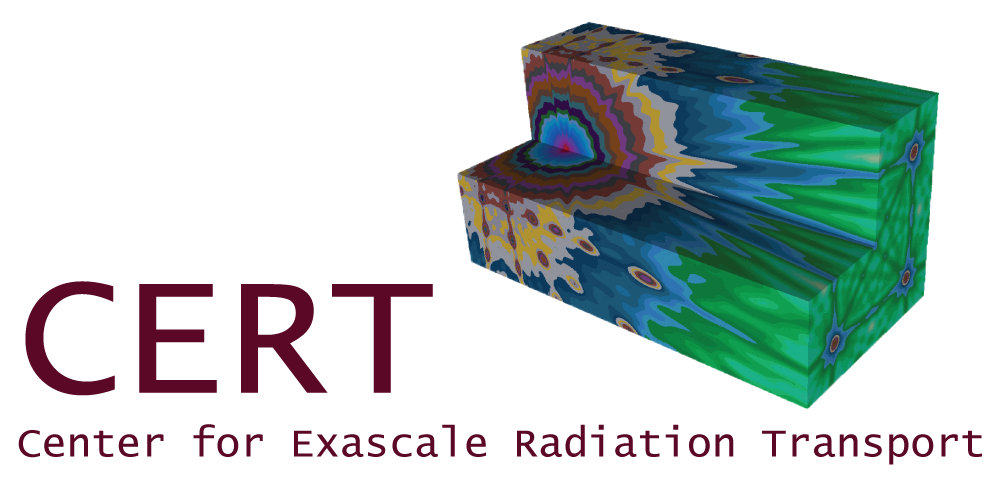
\includegraphics[height = 1cm,width=2cm]{figures/cert_logo_maroon.png}
	\end{textblock*}
}
\beamertemplatenavigationsymbolsempty



\begin{document}
%	

\title[Partitioning Optimization]{Partitioning Optimization for Massively Parallel Transport Sweeps on Unstructured Grids}
\author[Ghaddar]{Tarek Ghaddar}
\institute[TAMU]{Tarek Ghaddar \\ Chair: Jean Ragusa \\ Committee: Jim Morel, Marvin Adams, Nancy Amato}
\date[December 12, 2018]

{
\setbeamertemplate{headline}{}
\begin{frame}
\vspace{-1.1cm}
	\begin{figure}[t]
		\centering
			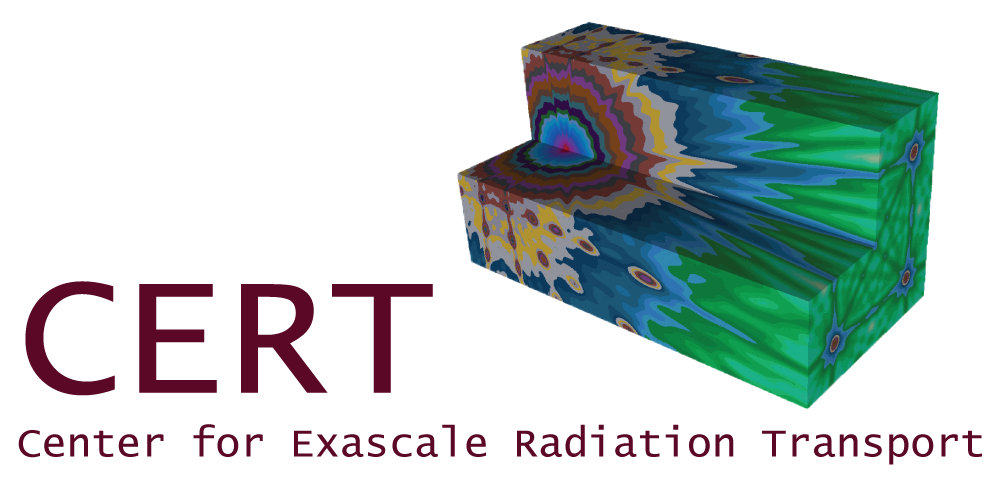
\includegraphics[width=.25\textwidth]{figures/cert_logo_maroon.png}
	\end{figure}
\vspace{-0.75cm}
\titlepage
\end{frame}
}

\setbeamertemplate{footline}
{

%\vspace{-0.1ex}
\begin{beamercolorbox}[wd=\textwidth,ht=3.5ex]{khumna}

\includegraphics[width = 0.95\textwidth]{figures/cert_banner.pdf}
	%\begin{textblock*}{10mm}(0.95\textwidth,10cm)
	\insertframenumber/\inserttotalframenumber
	%\end{textblock*}
\end{beamercolorbox}
%\begin{beamercolorbox}[wd=0.05\textwidth,ht=3.5ex]{khumna}

%\end{beamercolorbox}
}

\begin{frame}
\tableofcontents
\end{frame}

\section{Introduction and Previous Work}

\begin{frame}[t]\frametitle{Introduction}
\begin{block}{}
\begin{itemize}
	\item Massively parallel transport sweeps have been shown to scale up to 750,000 cores on logically cartesian grids.
	\item Structured meshes are somewhat limiting when attempting to simulate more complex problems and experiments.
	\item Unstructured meshes allow us to simulate realistic problems, but introduce unbalanced partitions. 
	\item PDT (Texas A\&M's massively parallel transport code) introduced two load balancing algorithms that repartition the mesh in order to obtain a roughly equivalent amount of cells per processor. 
	\item However, this can sacrifice the optimal sweep partitioning (cut lines all the way through the domain) in favor of balance. 
	\item The work proposed will balance perfect load balancing and optimal sweep partitioning in order to achieve the best possible time to solution.
\end{itemize}
\end{block}
\end{frame}

\begin{frame}[t]\frametitle{Load Balancing}
\begin{block}{Load Balance Metric}
  \begin{itemize}
    \item Max cells per subdomain divided by the average cells per subdomain:
      \begin{itemize}
        \item$f =\frac{\underset{ij}{\text{max}}(N_{ij})}{\frac{N_{tot}}{I\cdot J}}$
      \end{itemize}
    \item Column-wise metric: $f_I = \underset{i}{\text{max}}[\sum_{j} N_{ij}]/\frac{N_{tot}}{I}$
    \item Row-wise metric: $f_J = \underset{j}{\text{max}}[\sum_{i} N_{ij}]/\frac{N_{tot}}{J}$
    \item Per Column row-wise metric: $f_{J_i} = \text{max}[N_{ij}]_i/\frac{\sum_{j}N_{ij}}{J_i}$
  \end{itemize}		
  \tcr{Goal: minimize $f$ using locations of cut lines in X and Y}\\
    
  Subsequent improvement in algorithm: once dimension 1 has been balanced, balance dimension 2, then balance dimension 3 (\tcr{load balancing by dimension})
\end{block}
\end{frame}

\begin{frame}[t]\frametitle{No Load Balancing, f = 41.82}
\centering
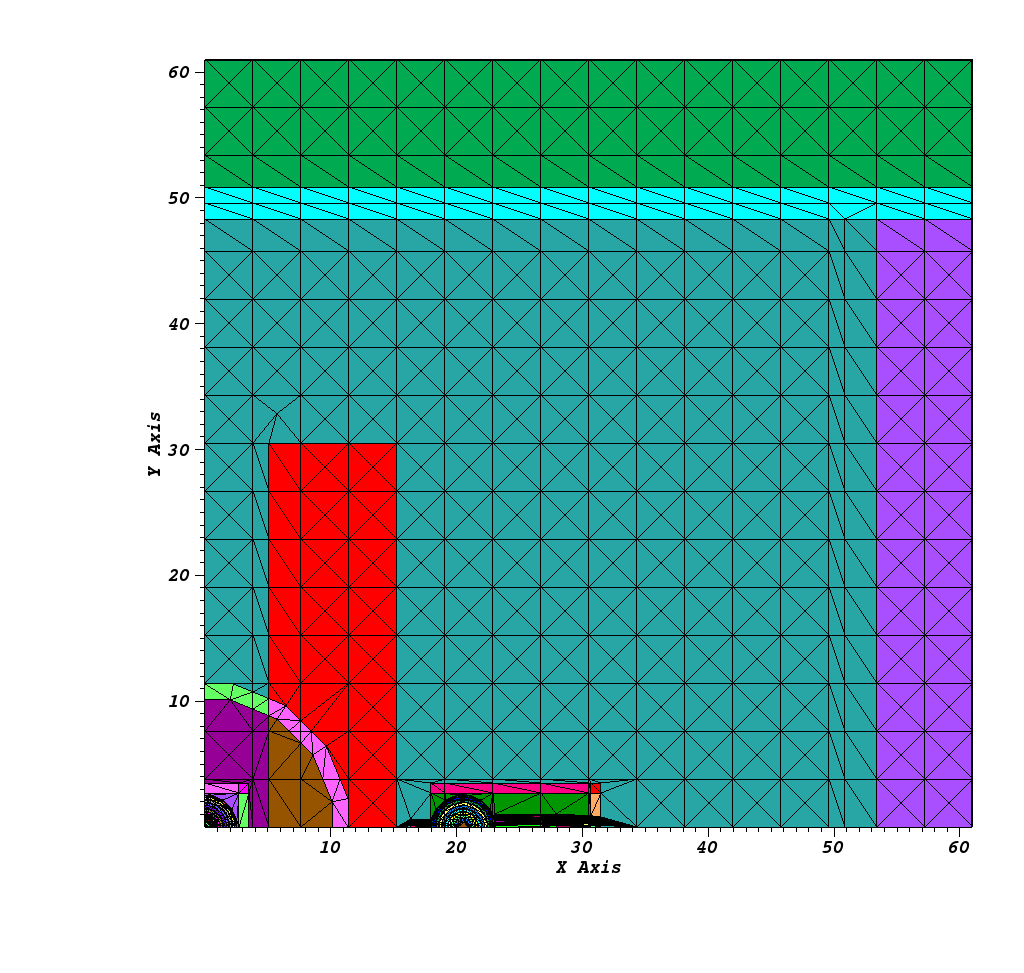
\includegraphics[scale=0.25]{figures/im12d_nolb.png}
\end{frame}

\begin{frame}[t]\frametitle{Load Balancing, f = 2.97}
\centering
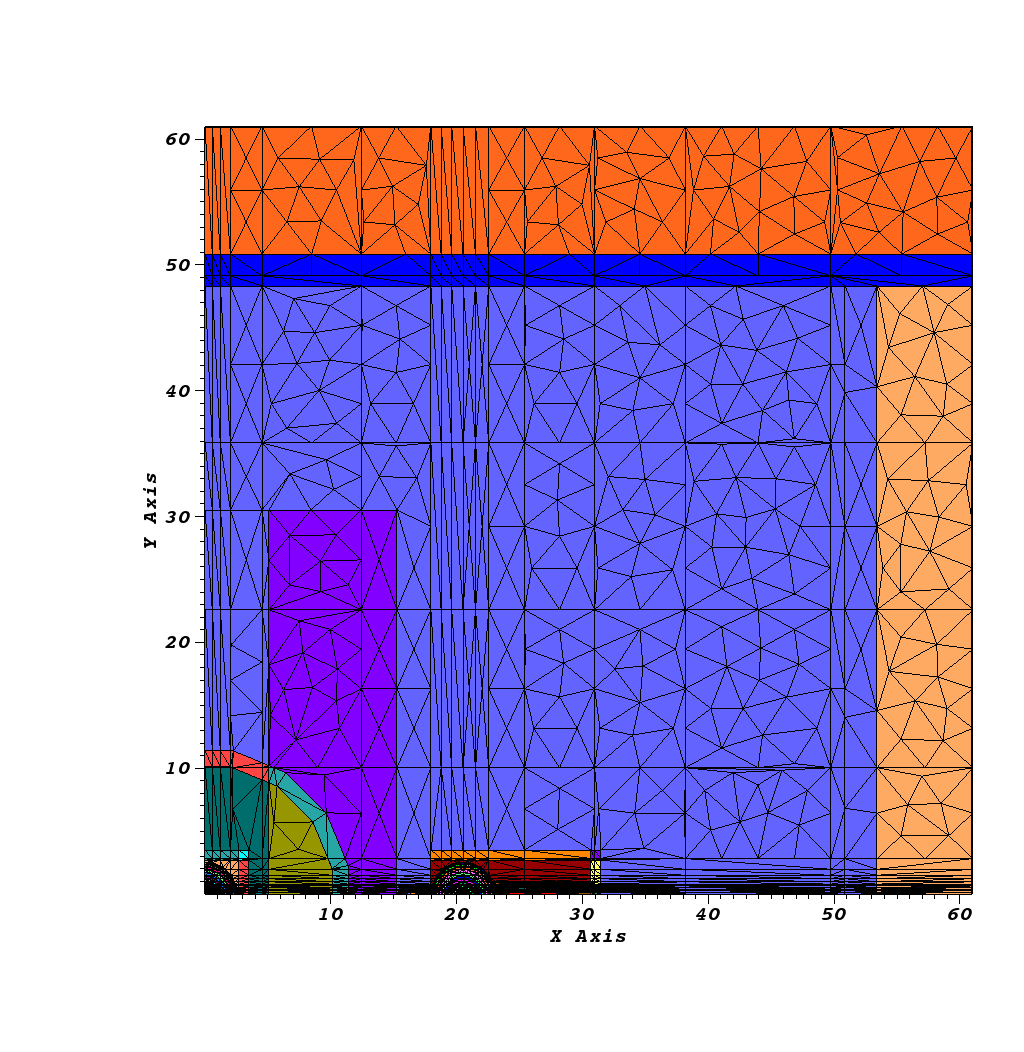
\includegraphics[trim={1cm 0cm 0cm 3cm},clip,scale=0.25]{figures/im12d_oldlb.png}
\end{frame}

\begin{frame}[t]\frametitle{Theoretical Motivation for LBD \\ (Courtesy of Dr. Adams)}
  \begin{block}{}
  \begin{itemize}
    \item Consider simple 2D layout with $M$ unaligned patches of high mesh density
    \item The cellset layout is $[M(N+1)+1] \times [M(N+1)+1]$ but only $MN^2$ cellsets have much work.
    \item Load Imbalance Factor $= \frac{\left( M(N+1)+1 \right)^2}{MN^2} \xrightarrow{N\to \infty} \frac{M^2N^2}{MN^2} = M$
  \end{itemize}
  \end{block}
  \begin{center}
    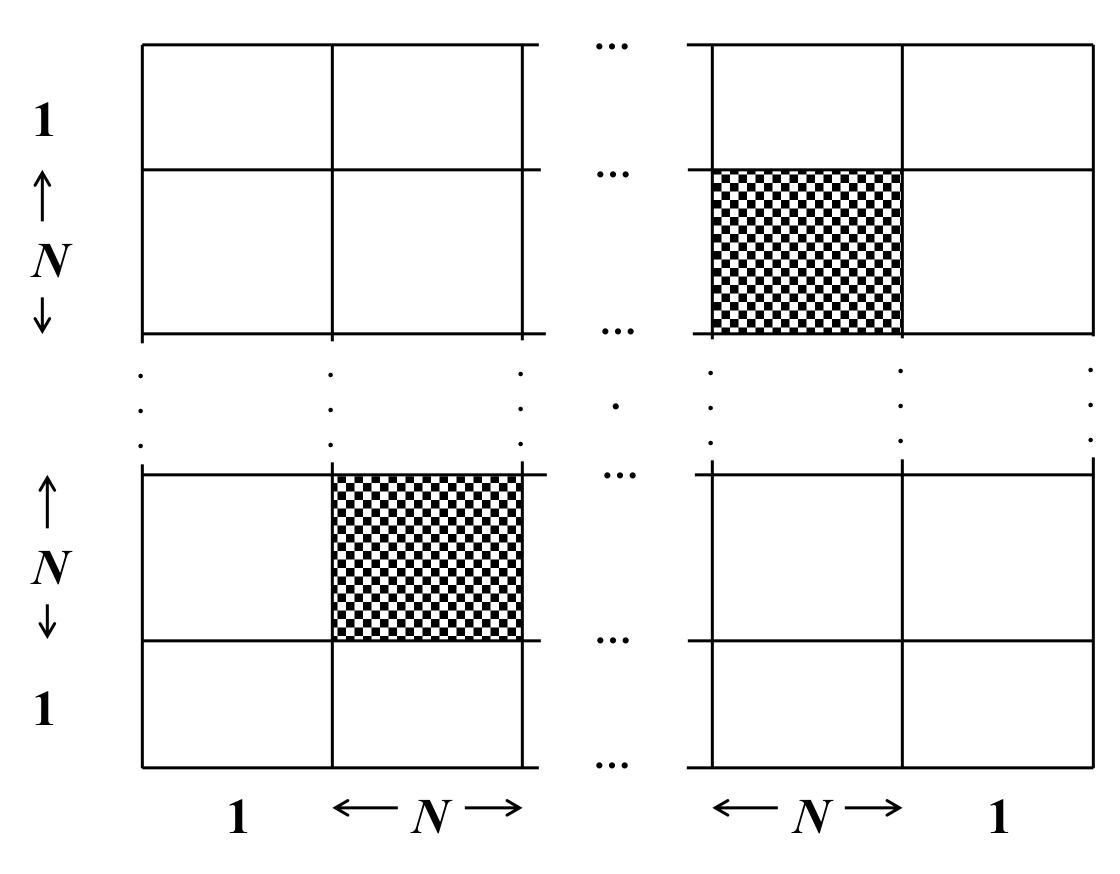
\includegraphics[width=5cm ]{figures/2dgeneral.png}
  \end{center}
\end{frame}

\begin{frame}[t]\frametitle{Load Balancing By Dimension, f = 2.02}
\centering
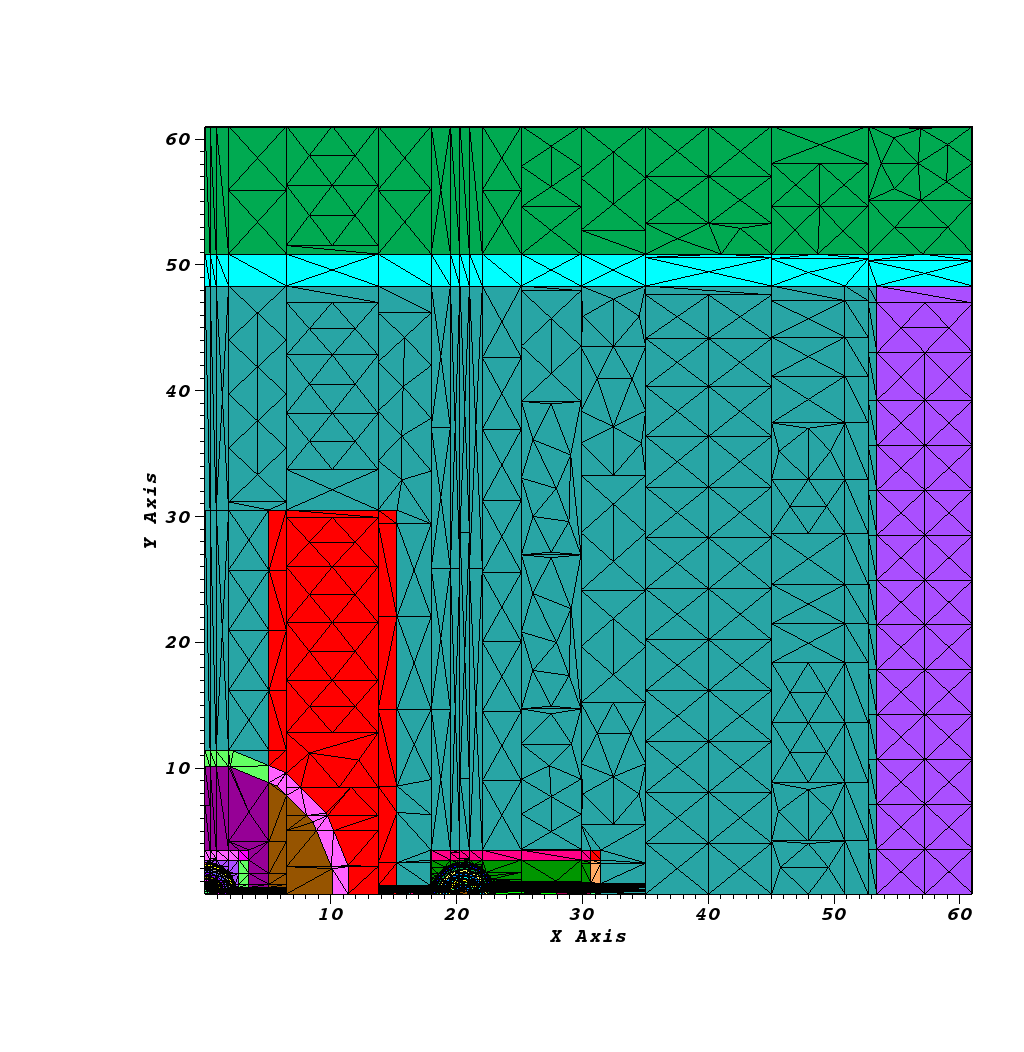
\includegraphics[scale=0.22]{figures/im12d_newlb.png}
\end{frame}

\begin{frame}[t]\frametitle{3D Load Balancing By Dimension}
\centering
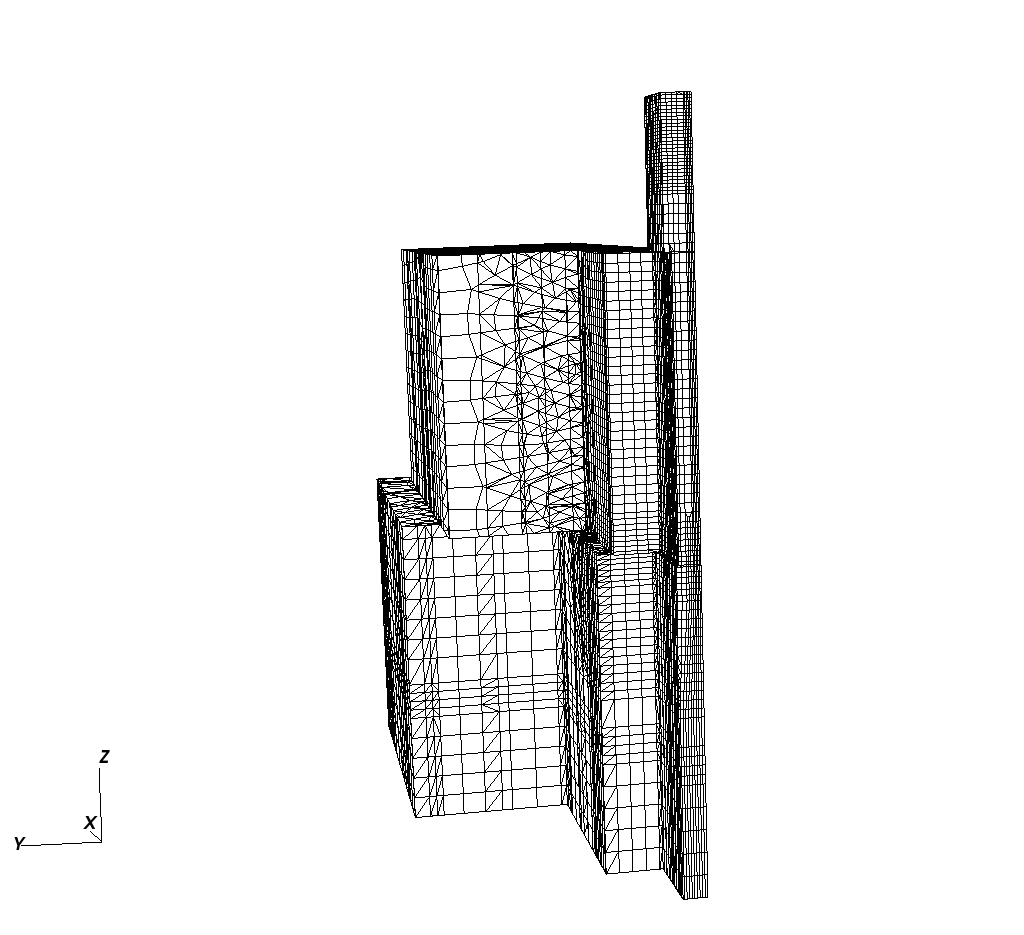
\includegraphics[trim={0cm 1cm 0cm 3cm},clip,scale=0.27]{figures/im1_foam_448.png}
\end{frame}

\begin{frame}[t]\frametitle{Consequences of Load Balancing By Dimension}
  \begin{block}{}
  \begin{itemize}
    \item Perfect load balance in some cases will come at the cost of optimal sweeping.
    \item Time to solution is the most important parameter, and if keeping a more optimal sweeping grid means a less balanced problem, then so be it.
    \item The concept of a stage may be misleading when dealing with imbalanced partitions, as we cannot easily characterize the idle time.
    \item A time-to-solution estimator must be built to more accurately predict sweep time.
  \end{itemize}
  \end{block}
\end{frame}

\begin{frame}[t]\frametitle{Sweep on Regular Grid with 3 Angle Sets}
	\animategraphics[loop,controls,width=0.8\linewidth]{10}{figures/sweep_figs/sweeps_png/sweep_regular_20x20_as3_dog/sweep_regular_20x20_as3_dog_}{1}{48}
	%\href{run:figures/sweep_figs/sweeps_png/sweep_regular_20x20_as3_dog/animation.gif}{Animation.gif}
\end{frame}

\begin{frame}[t]\frametitle{Sweep on LBD Grid with 3 Angle Sets}
	\animategraphics[loop,controls,width=0.8\linewidth]{10}{figures/sweep_figs/sweeps_png/sweep_random_20x20_as3_dog/sweep_random_20x20_as3_dog_}{1}{101}
	%\href{run:figures/sweep_figs/sweeps_png/sweep_random_20x20_as3_dog/animation.gif}{Animation.gif}
\end{frame}


\begin{frame}[t]\frametitle{Sweep on Worst Grid with 1 Angle Set}
	\animategraphics[loop,controls,width=0.8\linewidth]{10}{figures/sweep_figs/sweeps_png/sweep_worst_20x20_as1_dog/sweep_worst_20x20_as1_dog_}{1}{230}
	%\href{run:figures/sweep_figs/sweeps_png/sweep_worst_20x20_as1_dog/animation.gif}{Animation.gif}
\end{frame}

\section{Partitioning Optimization on Unstructured Grids}

\begin{frame}[t]\frametitle{Overview}
\begin{block}{}
\begin{itemize}
	\item We need to optimize the cut line location not for balance, but for the best possible sweep time.
	\item We must build a time-to-solution estimator that calculates the time to solution for a given cut line partitioning.
	\item The time to solution estimator will be fed into an optimizing function that minimizes the time to solution. The cut lines corresponding to the minimum time to solution are the optimal partitioning scheme.
\end{itemize}
\end{block}
\end{frame}

\begin{frame}[t]\frametitle{Time to Solution Estimator}
\begin{block}{}
\begin{itemize}
  \item For a given partition, this tool will build subset-level (not cell level) directed task dependence graphs for each octant, and weight the edges of that graph based on a set of criteria.
  \item The estimator returns the maximum time to sweep across one of the graphs.
  \item The maximum sweep time corresponds to the graph that has the maximum longest weighted path. 
\end{itemize}
\end{block}
\begin{block}{}
\begin{equation}
\text{TOS} = f(P_x, P_y, P_z, \text{\textcolor{red}{cut lines, threads}, machine params})
\end{equation}
\end{block}
\begin{block}{Important Assumption}
This process assumes that there are NO cycles in the TDGs. All graphs are acyclic.
\end{block}
\end{frame}

\begin{frame}[t]\frametitle{Longest Weighted Path}
\begin{block}{}
\begin{itemize}
	\item For a weighted directed graph, we look at all simple paths from the starting node to the ending node.
	\item The simple path that has the larger weight is the longest weighted path.
	\item We like the longest path because it reflects the sweep path that takes into account communication delays and waiting times for a single direction.
\end{itemize}
\end{block}
\end{frame}

\begin{frame}[t]\frametitle{Time to Solution Estimator}
\begin{block}{}
\begin{enumerate}
	\item Given a partitioning scheme (cut lines), build adjacency matrix.
	\item Build Directed Acyclic Graphs (DAGs) from the adjacency matrix, one for each octant.
	\item Weight the DAG's edges based on:
	\begin{itemize}
		\item Solve and communication time of each subset to its neighbors.
		\item Conflicts that arise between DAGs due to the sweep.
		\item This final edge weight reflects the amount of time it takes to solve the base node.
	\end{itemize}
	\item Compute solve time by getting the maximum edge-weighted sum of the longest paths for all DAGs.
\end{enumerate}
\end{block}
\end{frame}

\begin{frame}[t]\frametitle{Weighting the Graphs}
\begin{block}{}
\begin{itemize}
	\item In order to weight the graph properly, we need to have a mesh density function that we can calculate the cells (and then unknowns) per subset from.
	\item The weight of the edge between two nodes (subsets) in the graph represents the solve and communication time of the base node.
\end{itemize}
\end{block}
\begin{block}{}
\begin{align}
\text{cells per subset} &= \int_{\tcr{x_i}}^{\tcr{x_{i+1}}} \int_{\tcr{y_j}}^{\tcr{y_{j+1}}} \int_{\tcr{z_k}}^{\tcr{z_{k+1}}} \text{mesh density } dx dy dz \\
\label{weight}
\text{weight} &= N_u\cdot T_u (\text{\textcolor{red}{threads}}) + N_b\cdot T_{\text{comm}} + \text{latency}\cdot M_L \\
N_u &= \text{num cells}\cdot \text{unknowns per cell} \\
N_b &\approx(\text{num cells})^{\frac{2}{3}}\cdot \text{unknowns per boundary cell}
\end{align}
\end{block}
\end{frame}

\begin{frame}[t]\frametitle{Determining Cells per Subset}
	\centering
	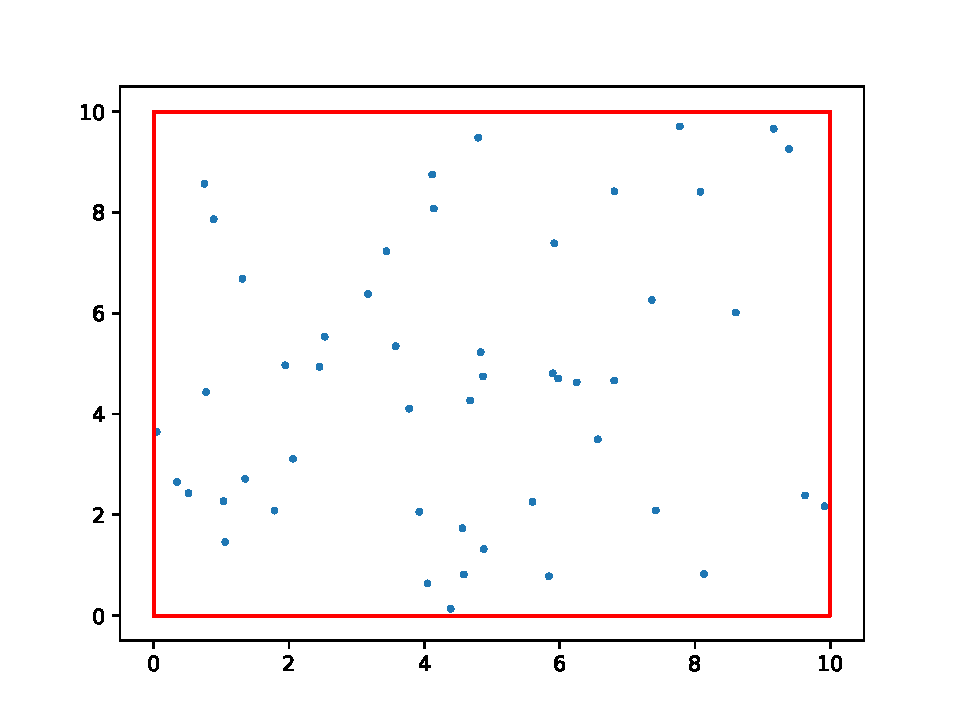
\includegraphics[scale=0.65]{figures/mesh_points.pdf}
\end{frame}

\begin{frame}[t]\frametitle{Determining Cells per Subset}
	\centering
	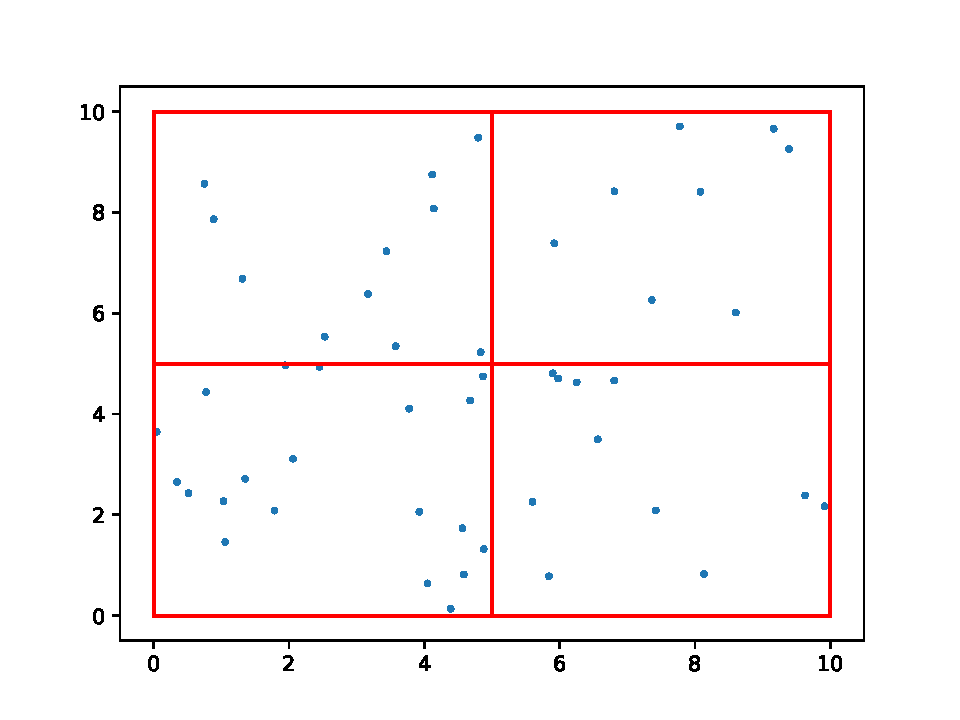
\includegraphics[scale=0.65]{figures/mesh_subsets.pdf}
\end{frame}

\begin{frame}[t]\frametitle{Determining Cells per Subset}
	\centering
	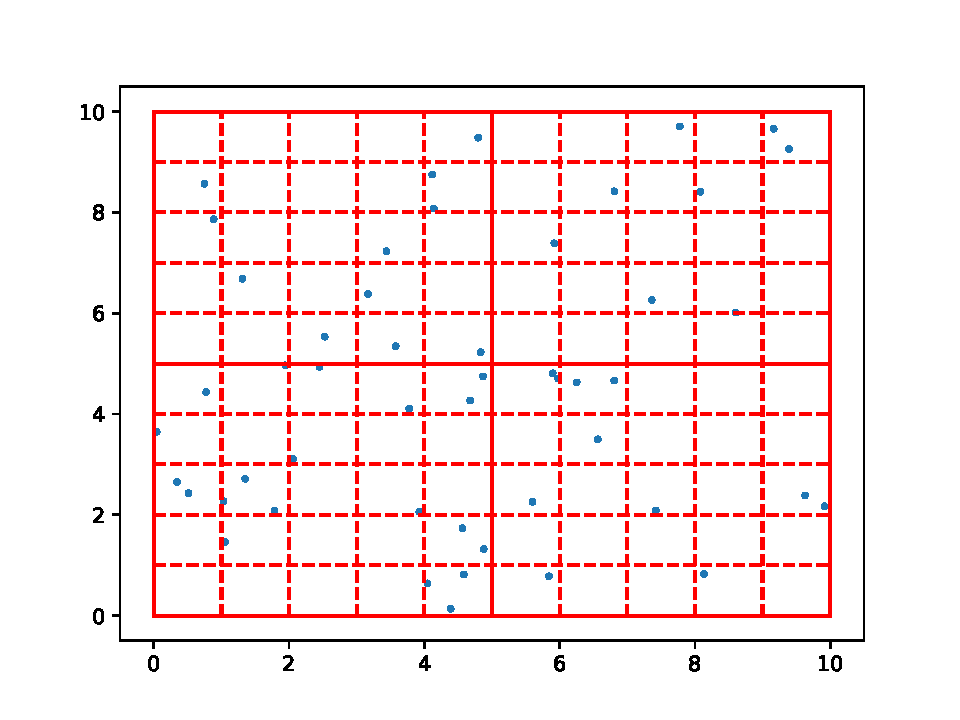
\includegraphics[scale=0.65]{figures/full_mesh_density.pdf}
\end{frame}

\begin{frame}[t]\frametitle{Conflict Detection and Resolution}
\begin{block}{}
\begin{itemize}
	\item Once all edges in all TDGs are appropriately weighted according to Eq. \ref{weight}, we need to detect and resolve sweep conflicts between the 8 octants.
	\item For perfectly balanced and optimally partitioned problems (structured grids) we will default to a depth-of-graph conflict resolution.
	\item For unbalanced partitions, we will default to a first come first serve conflict resolution.
    \item We check for conflicts only amongst the longest paths of each graph. This simplification takes into account the upstream dependencies of each node, without losing the accuracy of the time to sweep each graph.
\end{itemize}
\end{block}
\end{frame}

\begin{frame}[t]\frametitle{First Come First Serve Conflict Resolution}
\begin{block}{}
\begin{itemize}
	\item The first octant to arrive to a node will begin solving it, and the remaining octants will incur a delay (if applicable).
	\item The delay is reflected in each remaining TDG by adding the corresponding delay as a weight to the applicable edge.
	\item If two octants arrive to a node at the same time, the octant with the greater remaining depth-of-graph and priority octant wins the tie.
\end{itemize}
\end{block}
\begin{block}{Potential Future Work: hybrid depth-of-graph/first come first serve conflict resolution}
\begin{itemize}
	\item Two (or more) paths arrive to a node at different time, and when that node is free to solve, the path with the greater depth-of-graph remaining solves first.
\end{itemize}
\end{block}
\end{frame}

\begin{frame}[t]\frametitle{Conflict Detection}
	\centering
 	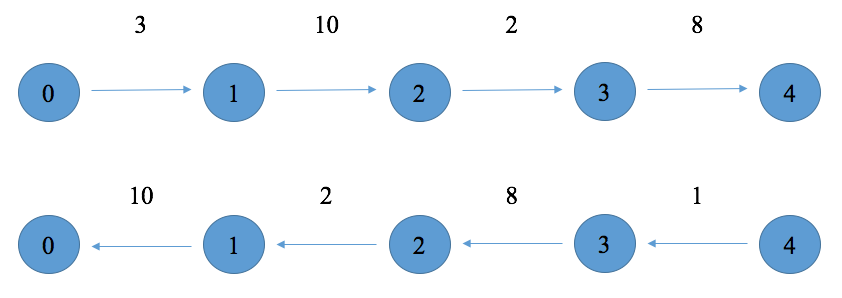
\includegraphics[scale=0.35]{figures/preconflict.png}
	
	\begin{block}{}
		\begin{itemize}
			\item A conflict arises at Node 1. The first path arrives at $t=3$, but takes 10 seconds to solve.
			\item The second path arrives at $t= 11$, while the first path is solving Node 1.
		\end{itemize}
	\end{block}
\end{frame}

\begin{frame}[t]\frametitle{Conflict Resolution}
	\centering
	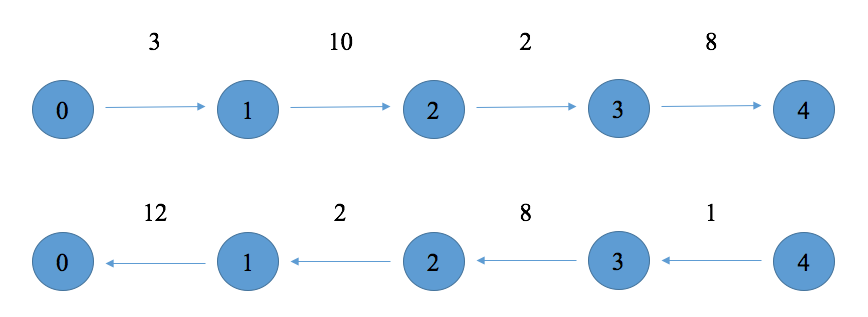
\includegraphics[scale=0.35]{figures/postconflict.png}
	
	\begin{block}{}
	\begin{itemize}
		\item The second path waits 2 seconds to solve Node 1.
		\item This delay is added to the edge weight between Node 1 and Node 0 to reflect the new total solve time for Node 1 in the second path.
	\end{itemize}
	\end{block}
	
\end{frame}

\begin{frame}[t]\frametitle{General Conflict Resolution Algorithm}
\begin{algorithm}[H]
\begin{algorithmic}[1]
\FOR{$g = 1$ to $G-1$}
\FOR{$node = 1$ to $N$}
\STATE Find fastest path to $node$
\STATE Add delays to slower paths
\STATE Remove fastest path to $node$ for future iterations
\ENDFOR
\ENDFOR	
\label{conflict}
\end{algorithmic}
\end{algorithm}

\begin{block}{}
\begin{itemize}
	\item $G$ is the total number of DAGs.
	\item N is the total number of nodes per DAG.
	\item It is necessary to have $G-1$ iterations so that slower paths to each node will address conflicts with each other. This will be illustrated in the test case shown.
\end{itemize}
\end{block}
\end{frame}

\begin{frame}[t]\frametitle{Sweeping the Graph}
\begin{block}{}
\begin{itemize}
	\item Now that all TDGs are weighted based on solve time, communication time, and delays, we can easily calculate the time it takes each octant to sweep across the graph. 
	\item The sum of the  longest path's edge weights in each graph represents the time each octant takes to complete its sweep.
	\item The maximum weighted edge sum of these longest paths is the estimated time to solution that we use.
\end{itemize}
\end{block}
\end{frame}

\section{Preliminary Results and Setbacks}

\begin{frame}[t]\frametitle{Uniform Unbalanced Test (2D)}
\centering
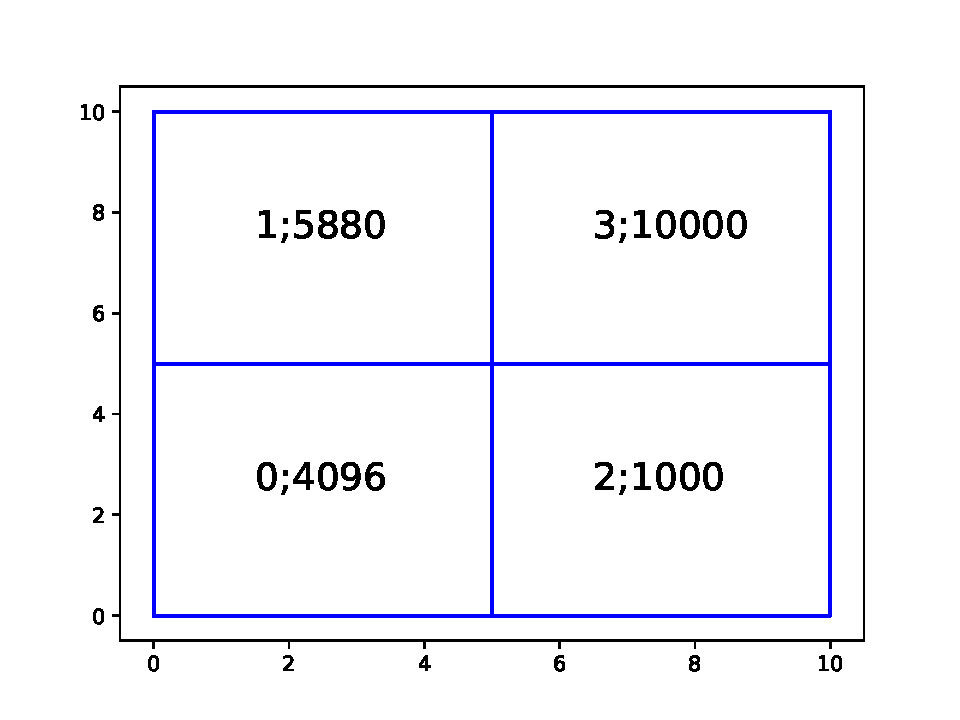
\includegraphics[trim={1cm 0cm 1cm 1cm},clip,scale=0.75]{figures/2d_layer.pdf}
\end{frame}

\begin{frame}[t]{Longest Paths per Quadrant}
\begin{block}{}
	\begin{enumerate}
		\item 0,1,3
		\item 1,3,2
		\item 2,3,1
		\item 3,1,0
	\end{enumerate}
\end{block}
On future slides you will see a dummy node with the label "-1".
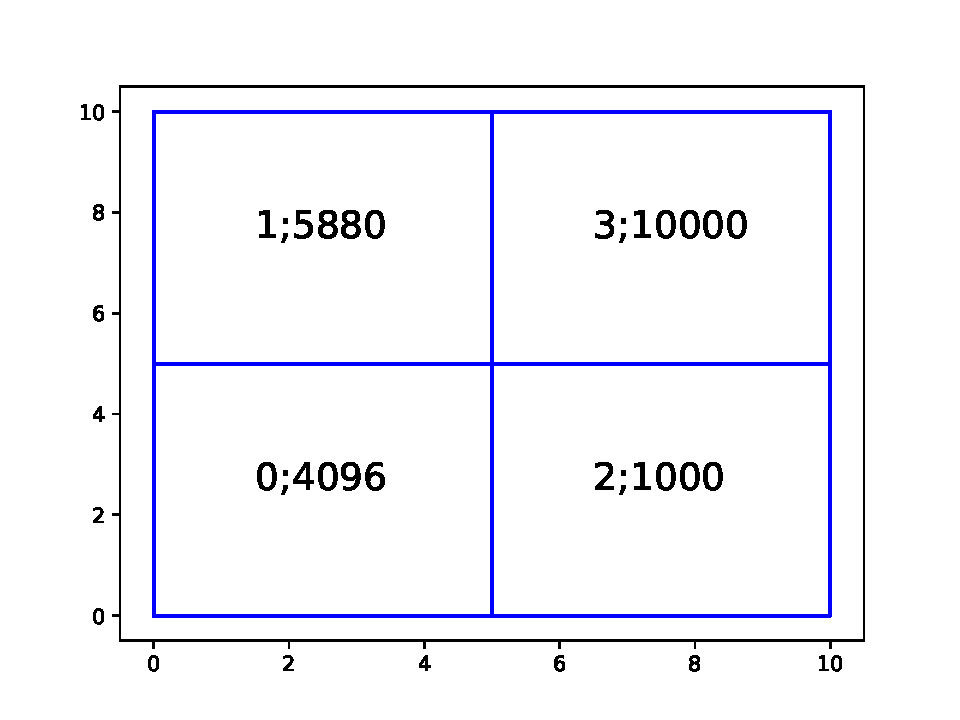
\includegraphics[trim={1cm 0cm 1cm 1cm},clip,scale=0.4]{figures/2d_layer.pdf}
\end{frame}

\begin{frame}[t]{Graph Weights with Solve and Comm. Time Only}
\centering
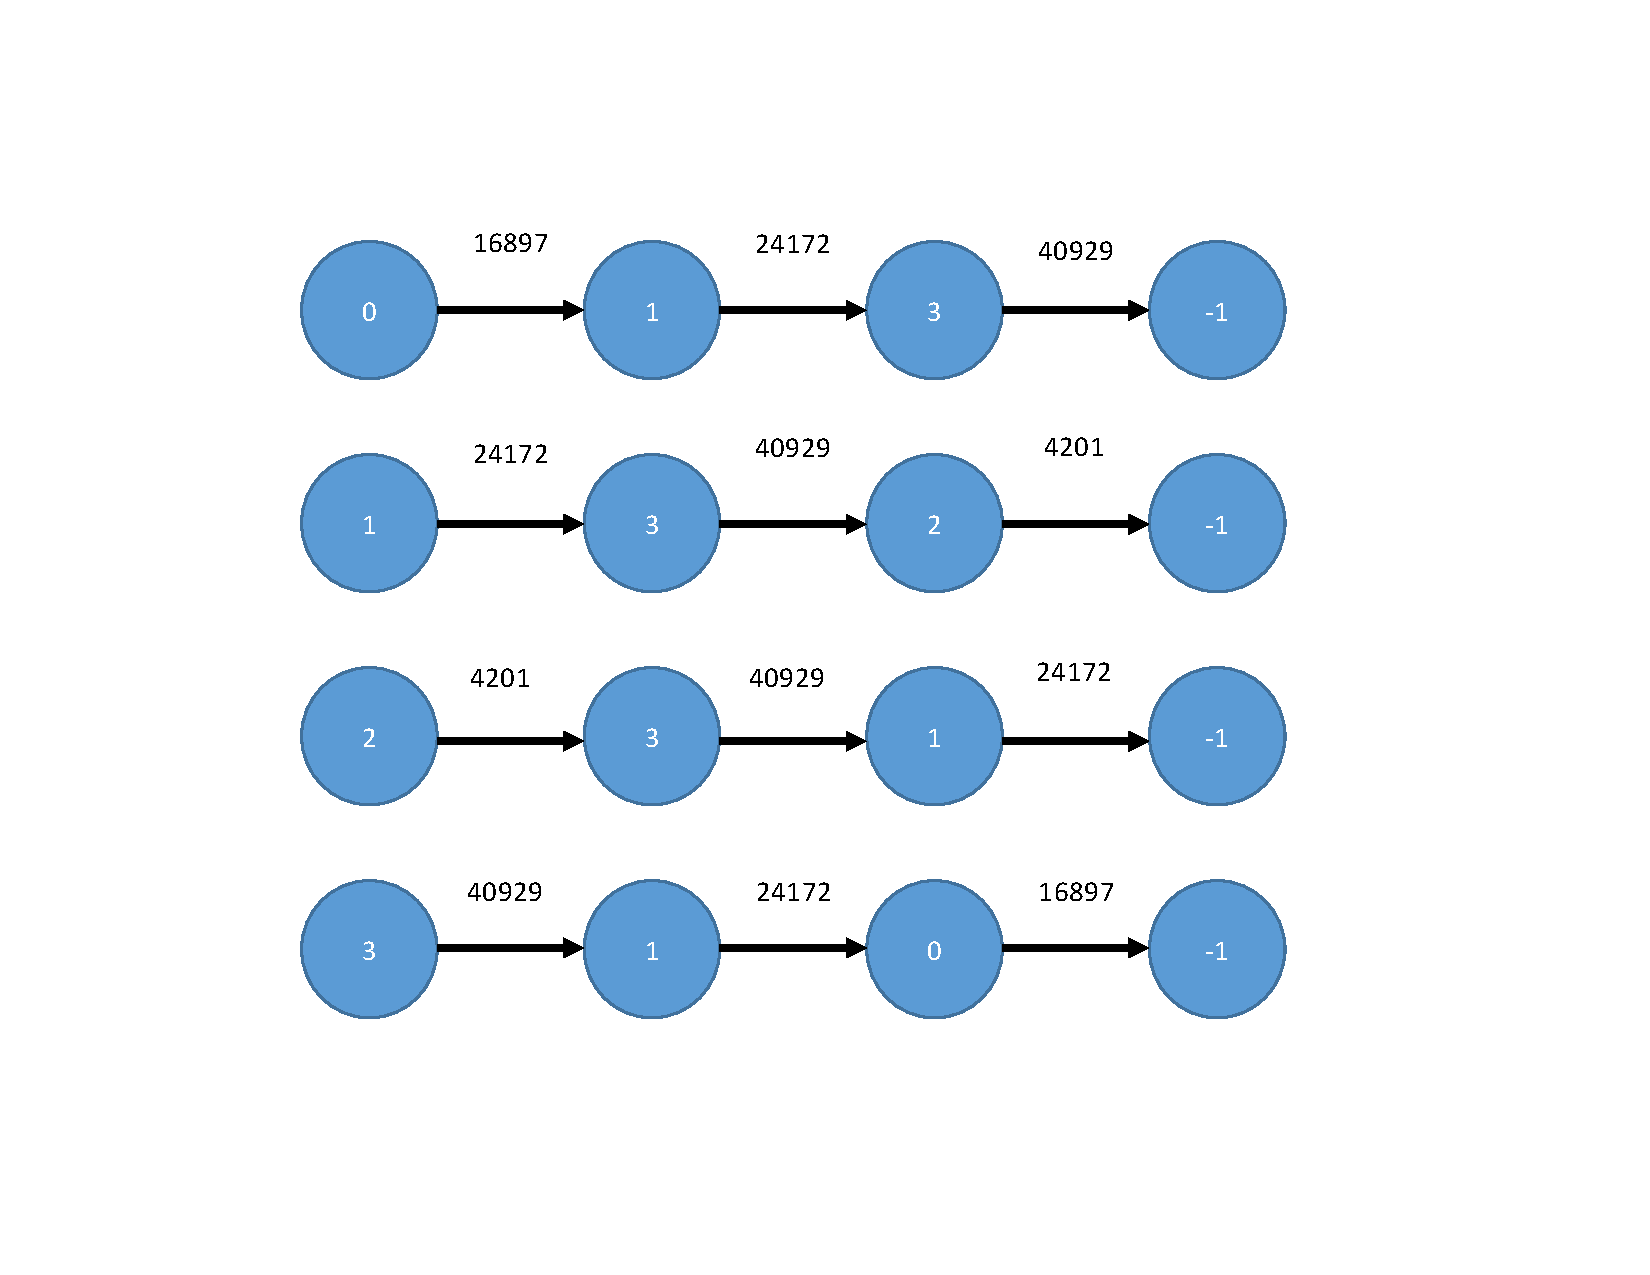
\includegraphics[trim={2cm 2cm 4cm 2cm},clip,scale=0.45]{figures/solve_only.pdf}
\end{frame}

\begin{frame}[t]{Conflicts at Iteration 0}
\centering
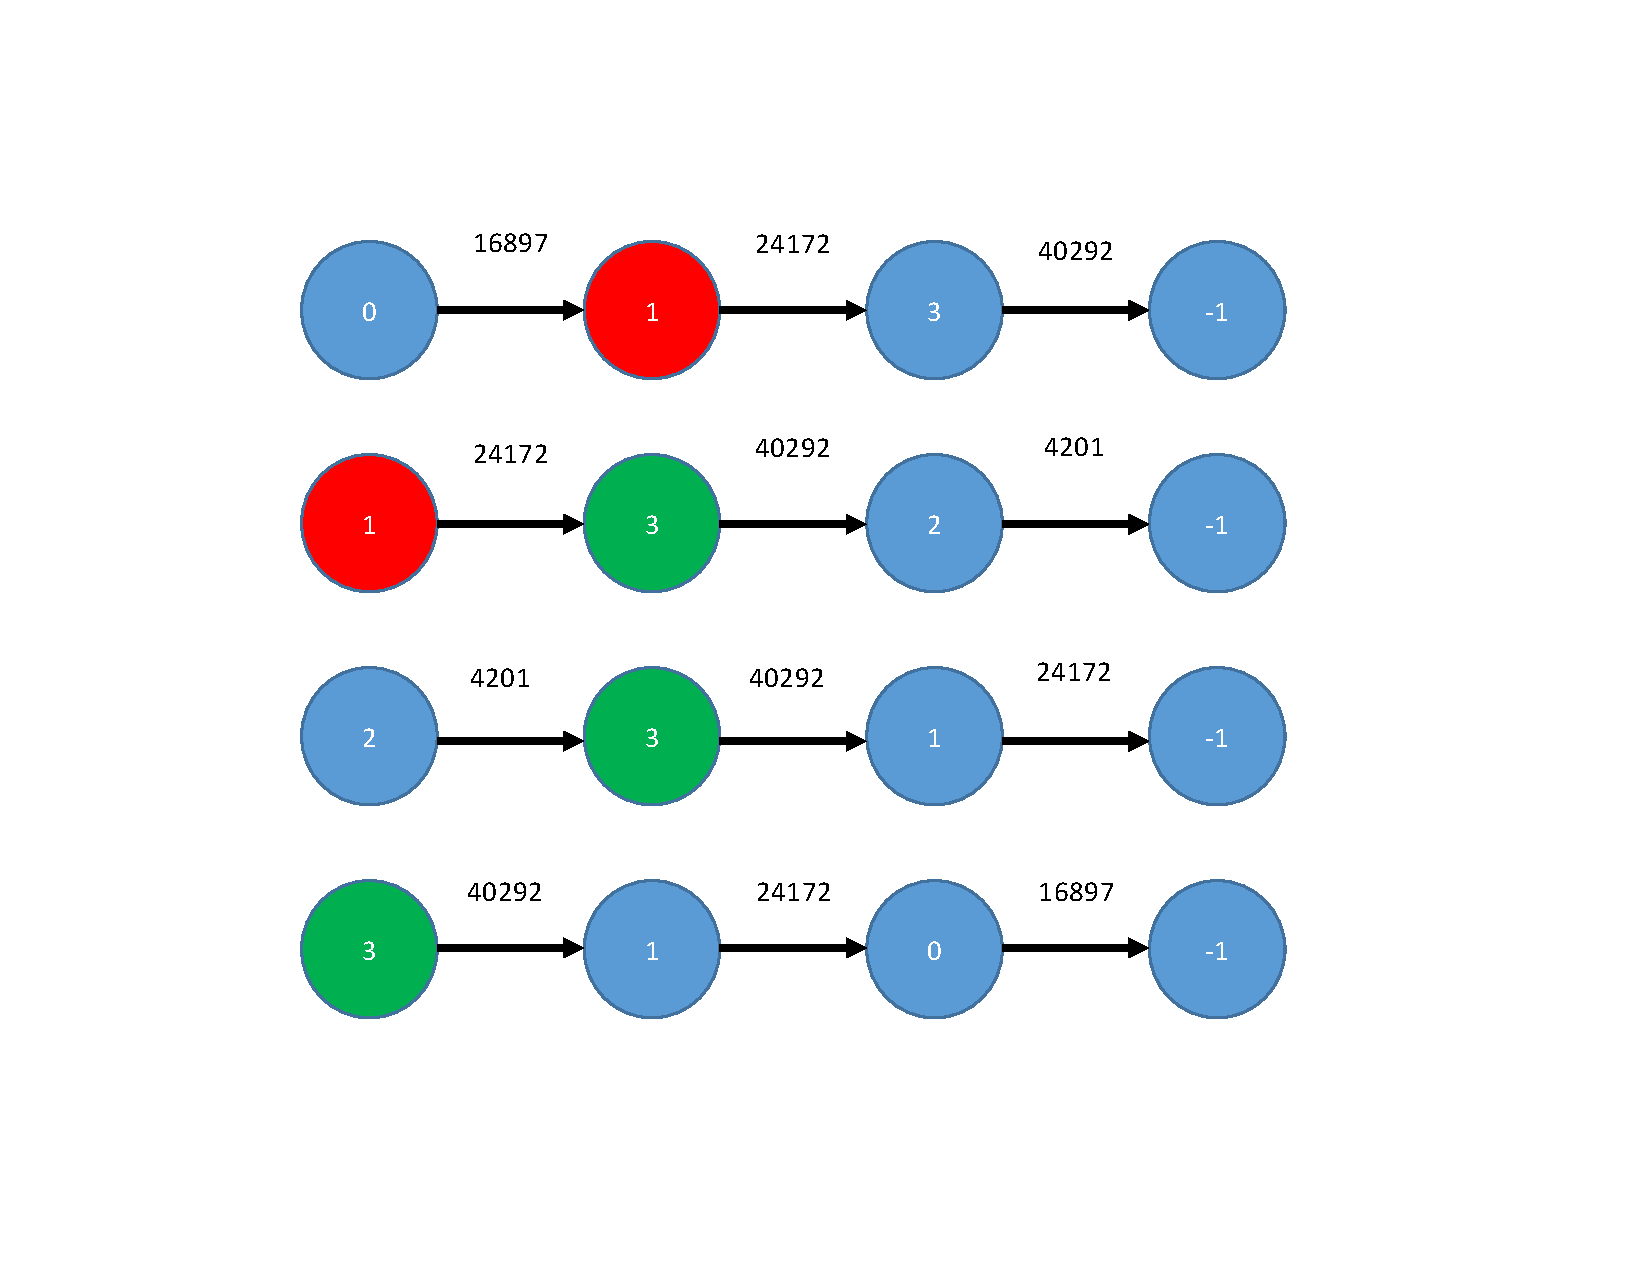
\includegraphics[trim={2cm 2cm 4cm 2cm},clip,scale=0.45]{figures/solve_only_conflicts.pdf}
\end{frame}

\begin{frame}[t]{Resolving Iteration 0}
\centering
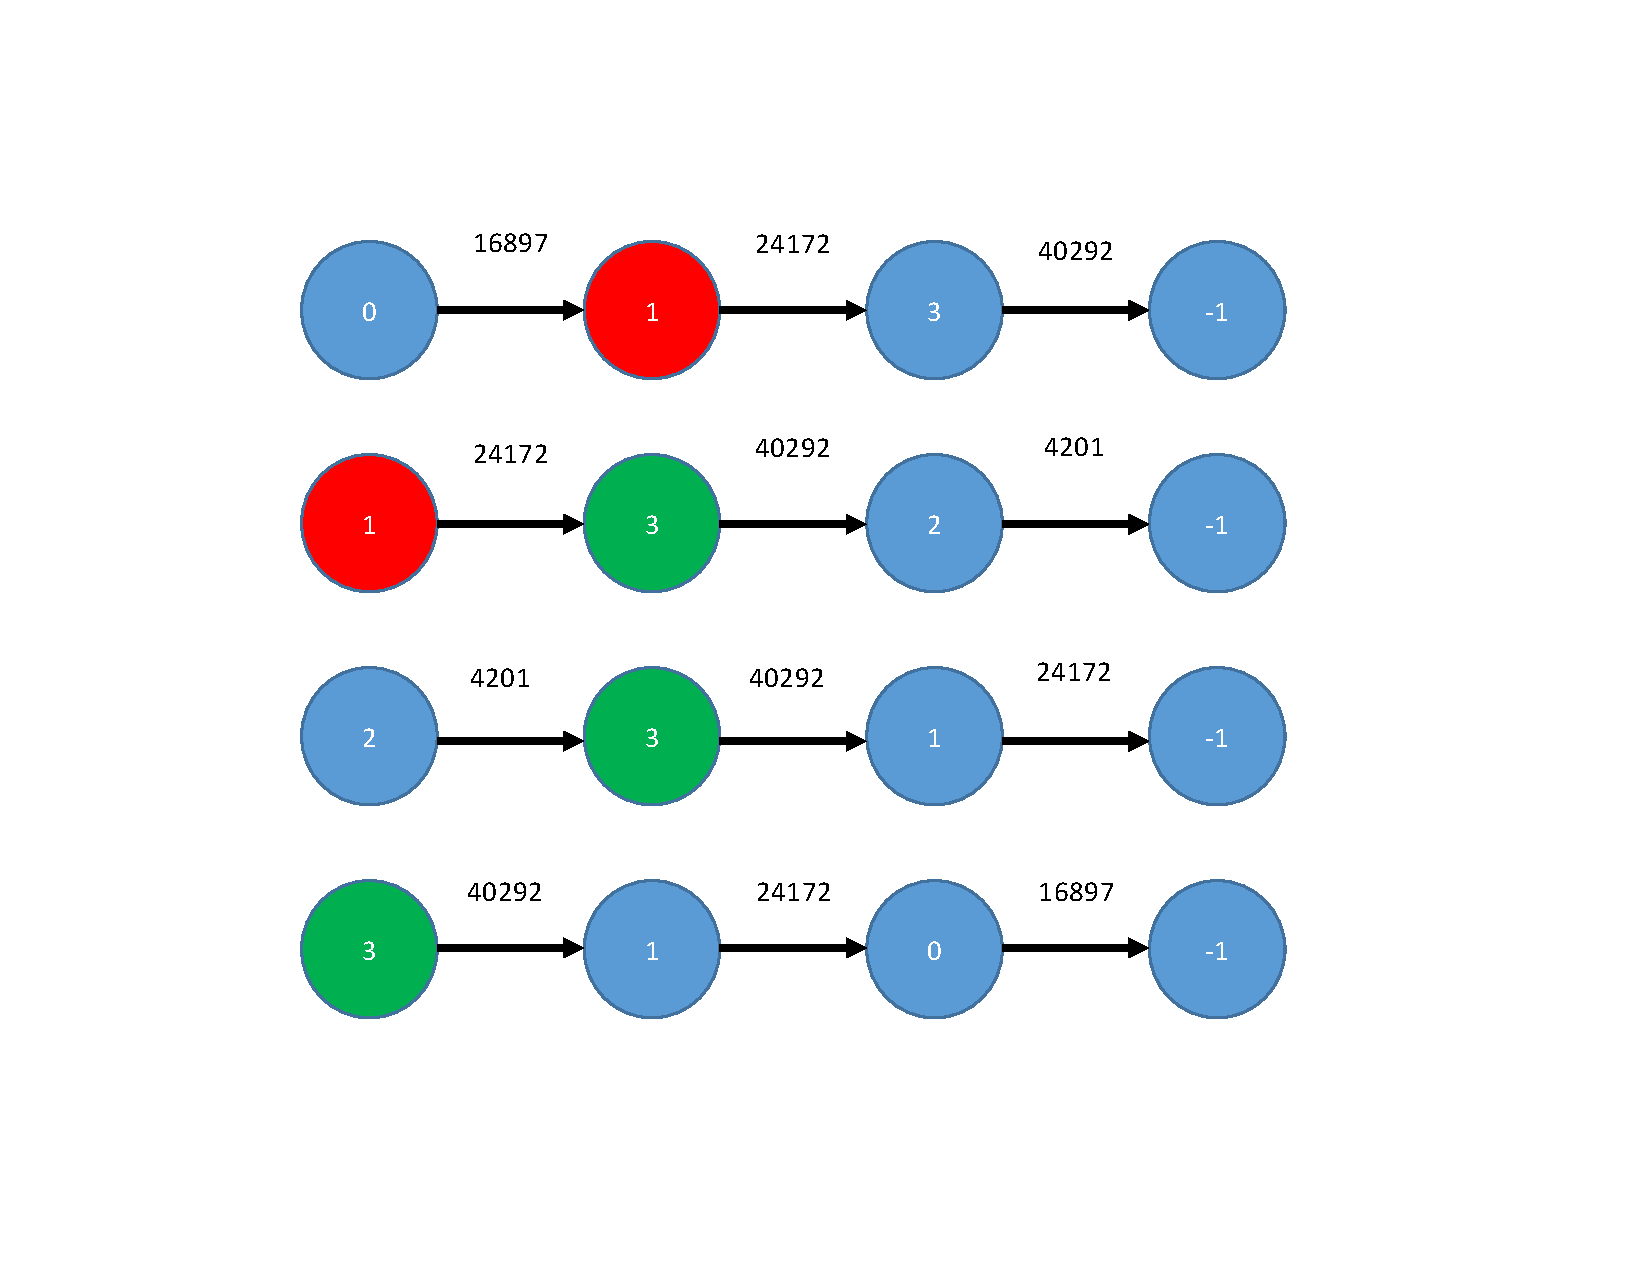
\includegraphics[trim={2cm 2cm 4cm 2cm},clip,scale=0.2]{figures/solve_only_conflicts.pdf}
\begin{block}{}
\begin{itemize}
\item There are no conflicts at Node 0 or Node 2. The fastest paths finish by the time the slower paths arrive.
\item Path 1 is still solving Node 1 when Path 0 arrives. Delay of $24172-16897=7275$ added to Path 0.
\item Paths 1 and 2 arrive at Node 3 before Path 3 finishes solving. Delays of $40929-24172=16757$ and $40929-4201=36728$  are added.
\end{itemize}
\end{block}
\end{frame}

\begin{frame}[t]{Iteration 1}
\centering
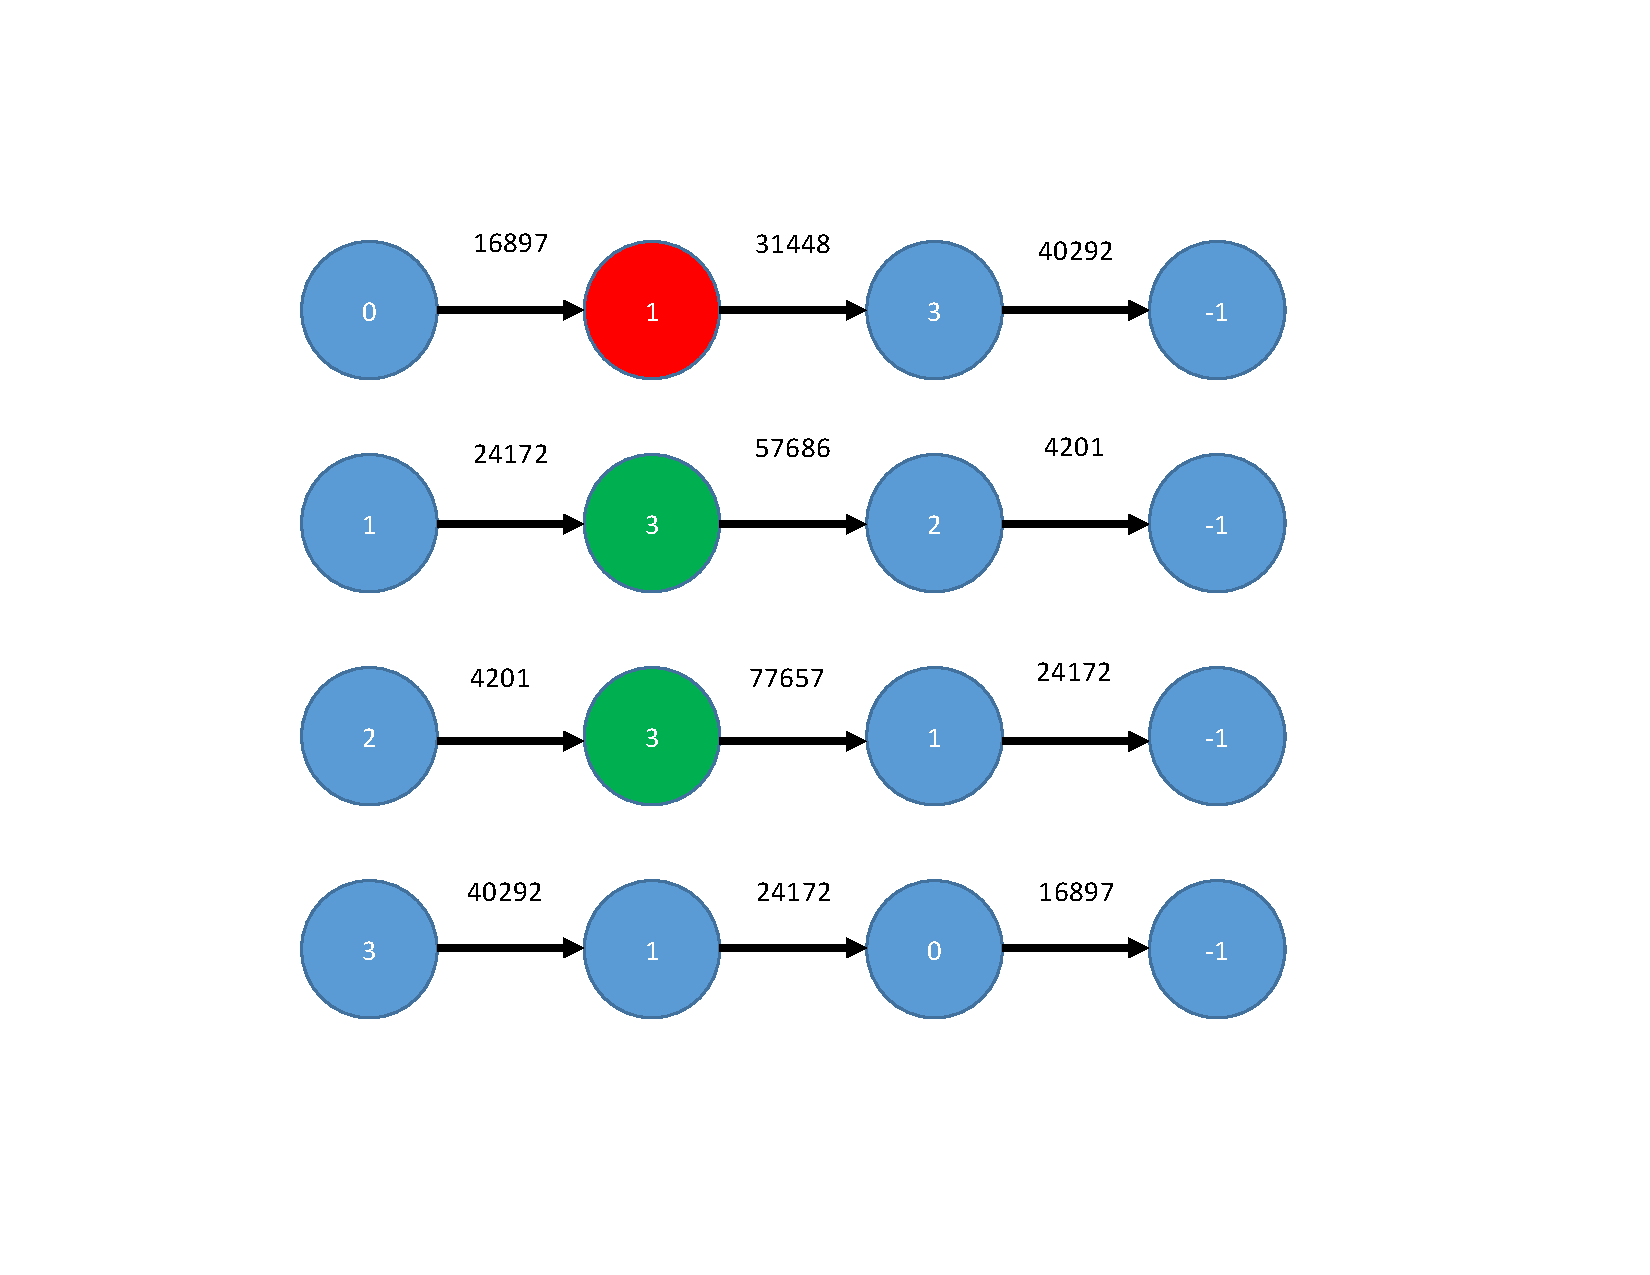
\includegraphics[trim={2cm 2cm 4cm 2cm},clip,scale=0.45]{figures/iteration1.pdf}
\end{frame}

\begin{frame}[t]{Conflicts at Iteration 1}
\centering
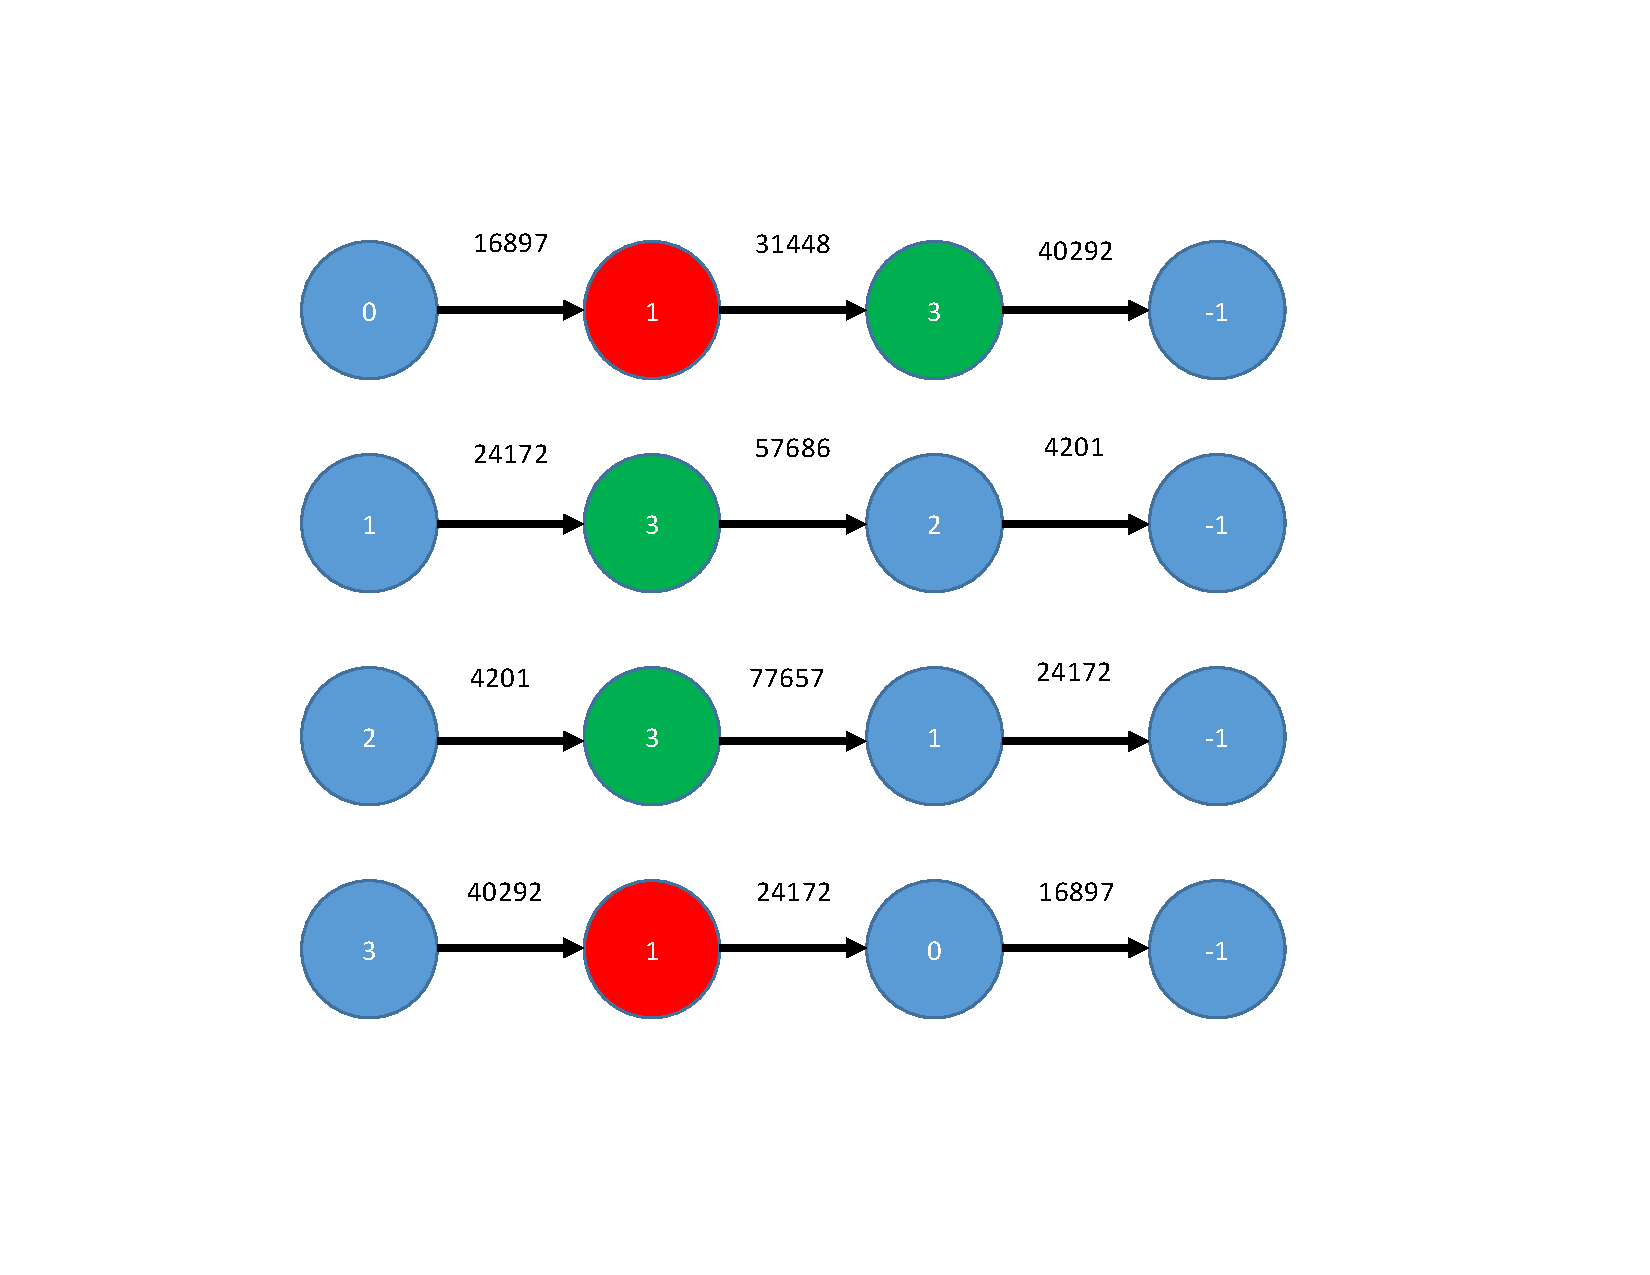
\includegraphics[trim={2cm 2cm 4cm 2cm},clip,scale=0.45]{figures/iteration1_conflicts.pdf}
\end{frame}

\begin{frame}[t]{Resolving Iteration 1}
\centering
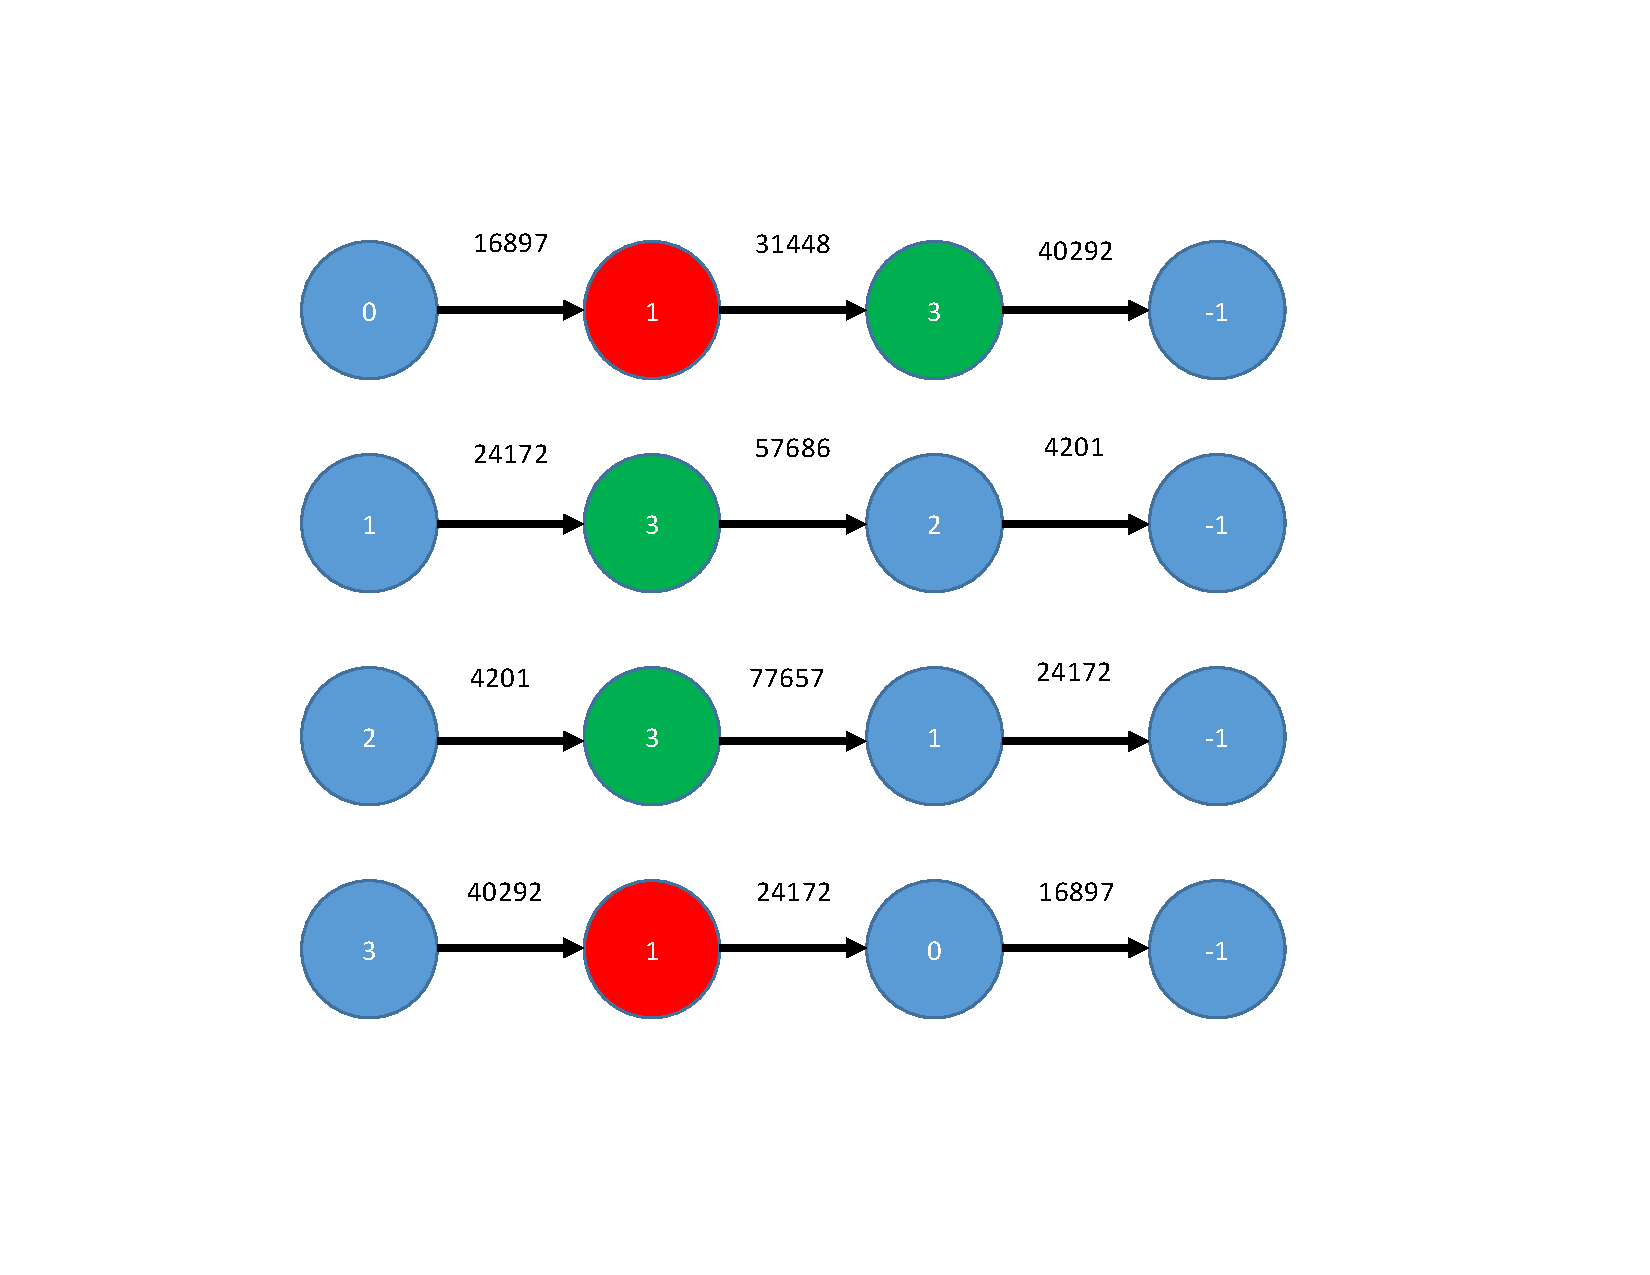
\includegraphics[trim={2cm 2cm 4cm 2cm},clip,scale=0.2]{figures/iteration1_conflicts.pdf}
\begin{block}{}
\begin{itemize}
\item Still no conflicts at Node 0 or Node 2.
\item Path 1 is still solving Node 1 when Path 3 arrives. Delay of $48345-40292=7416$ is added.
\item Path 2 starts solving Node 3 at t=40929. Path 1 is delayed a further 40929 (Node 3's solve time). 
\item Path 0 can solve Node 3 at t=48345. Path 2 is not finished solving until t=81858. Delay of $81858-48345=33513$ added.
\end{itemize}
\end{block}
\end{frame}

\begin{frame}[t]\frametitle{Iteration 2}
\centering
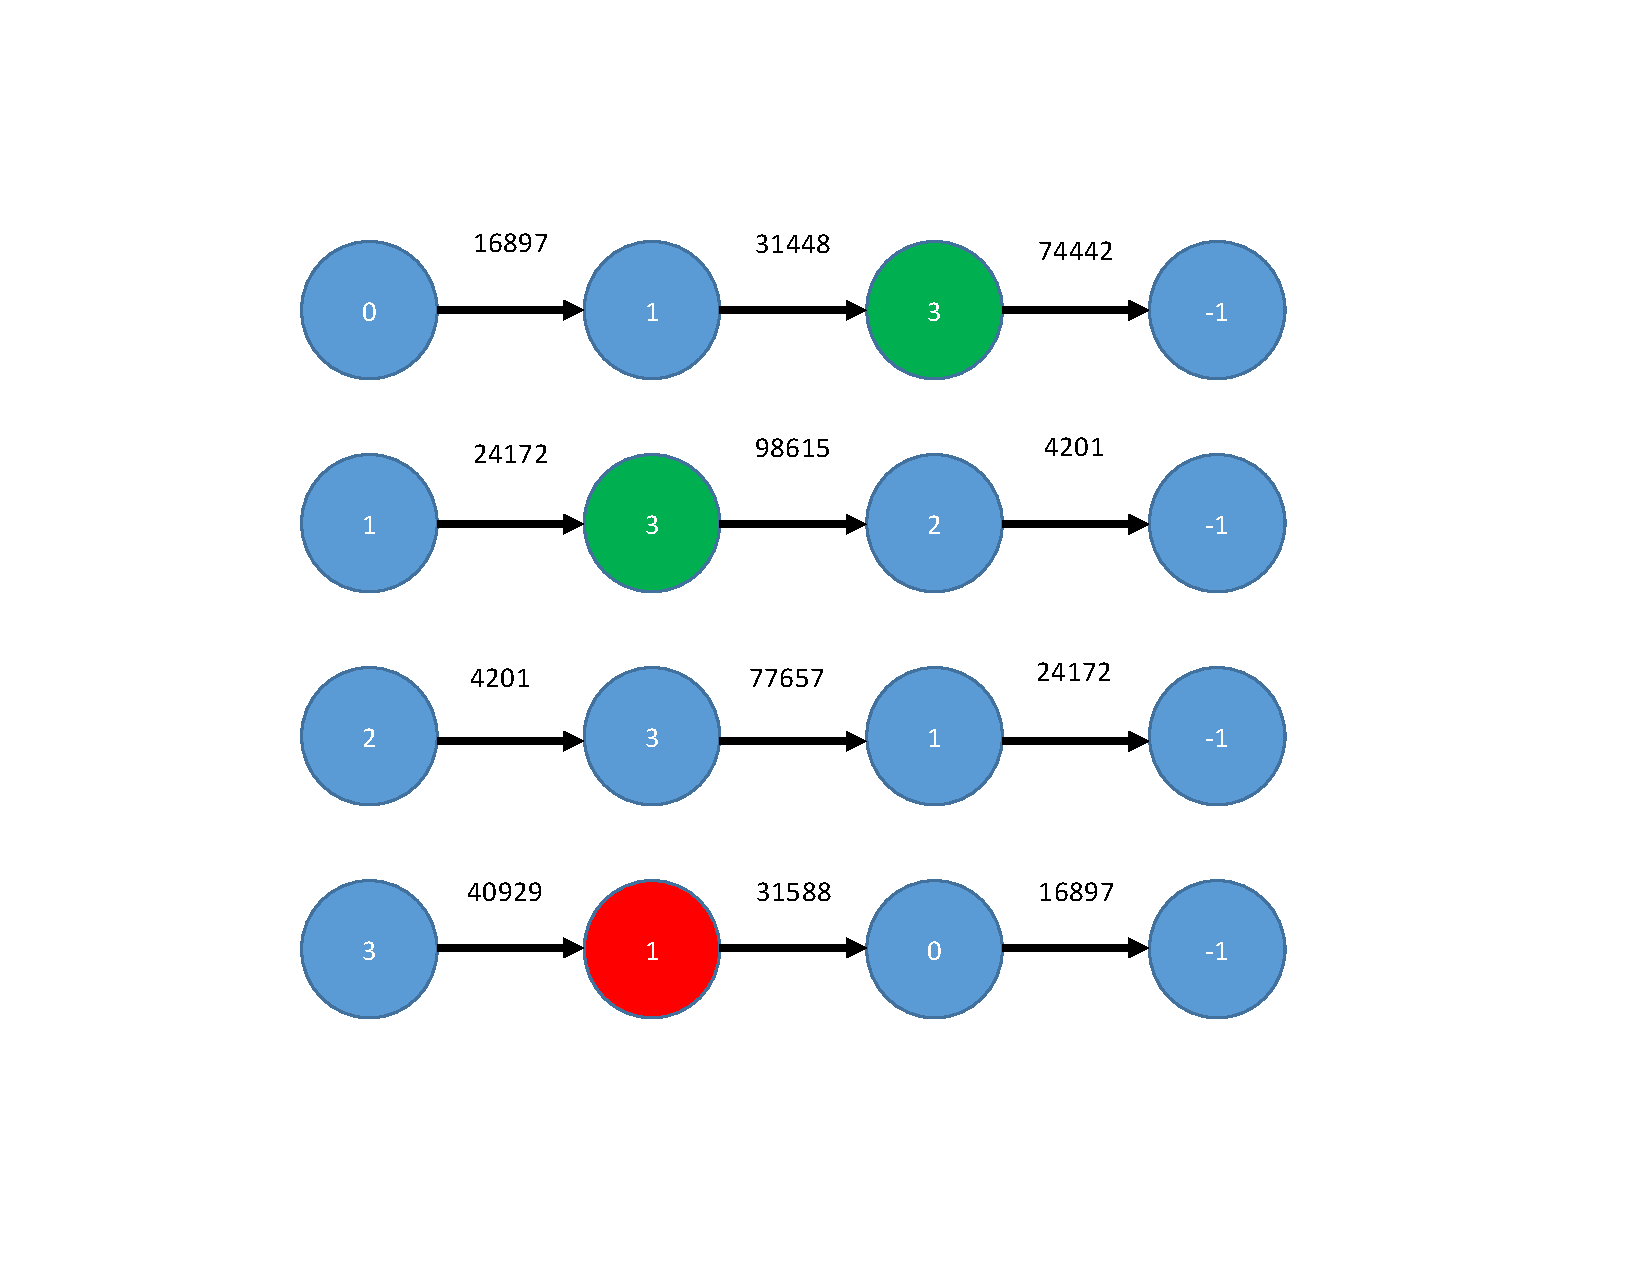
\includegraphics[trim={2cm 2cm 4cm 2cm},clip,scale=0.45]{figures/iteration2.pdf}
\end{frame}

\begin{frame}[t]{Conflicts at Iteration 2}
\centering
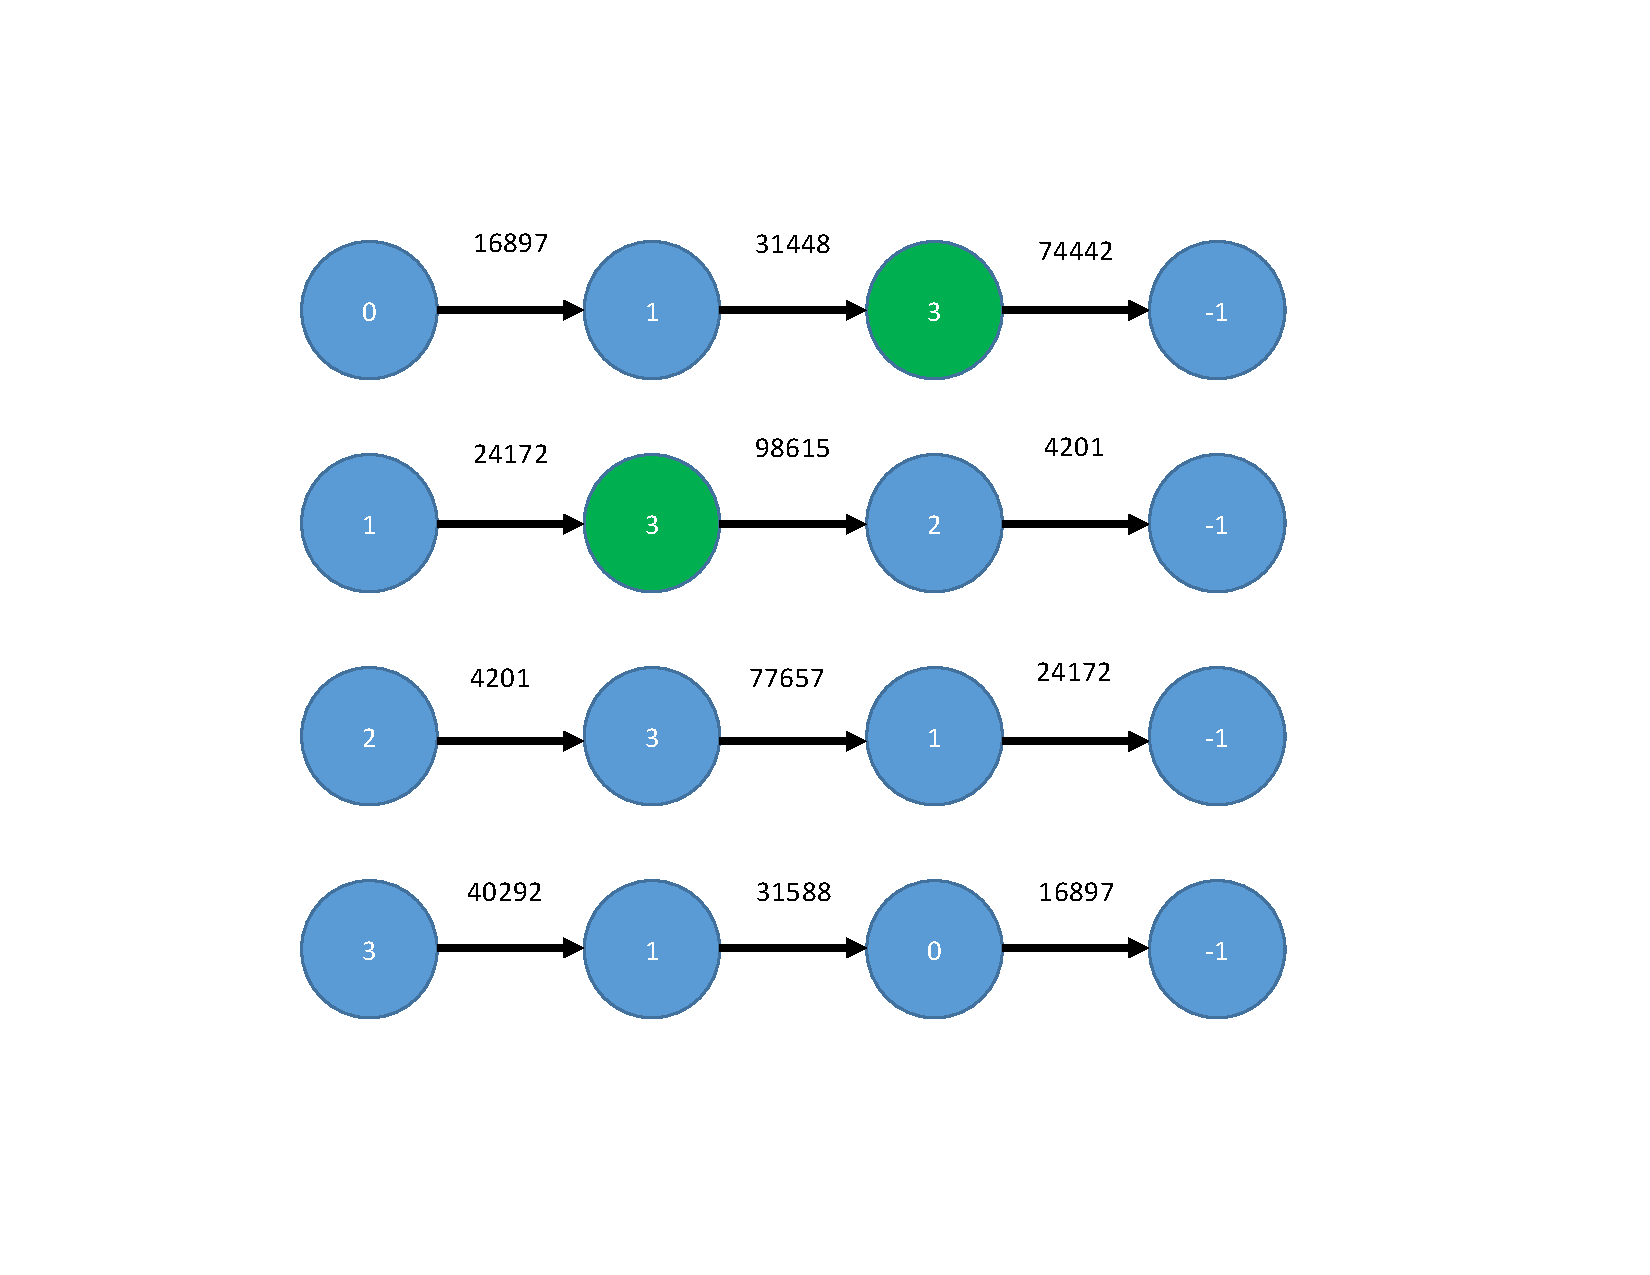
\includegraphics[trim={2cm 2cm 4cm 2cm},clip,scale=0.45]{figures/iteration2_conflicts.pdf}
\end{frame}

\begin{frame}[t]{Resolving Iteration 2}
\centering
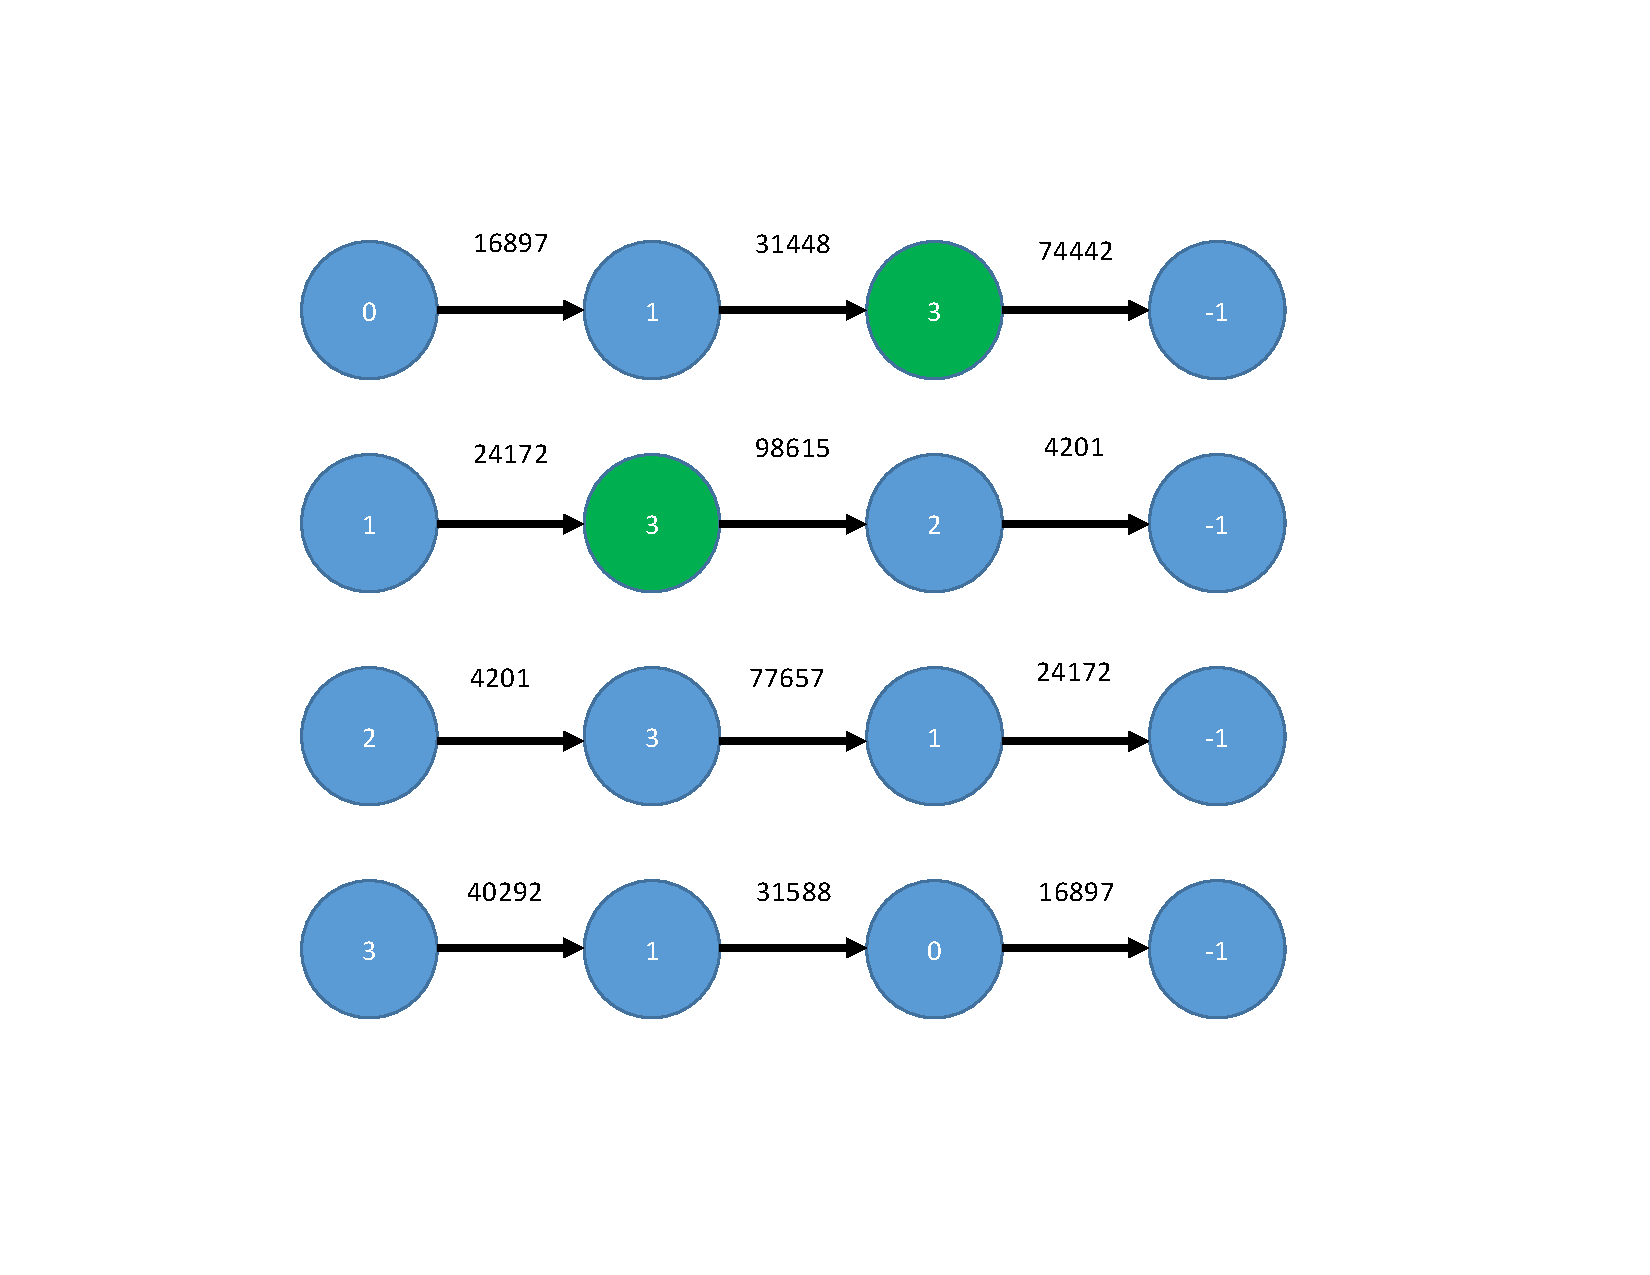
\includegraphics[trim={2cm 2cm 4cm 2cm},clip,scale=0.2]{figures/iteration2_conflicts.pdf}
\begin{block}{}
\begin{itemize}
	\item No conflicts at Nodes 0,1, or 2.
	\item Path 1 is done solving Node 3 at t=122787. Path 2 is delayed a further 40929 (Node 3's solve time).
\end{itemize}
\end{block}
\end{frame}

\begin{frame}[t]{Final Weights}
\centering
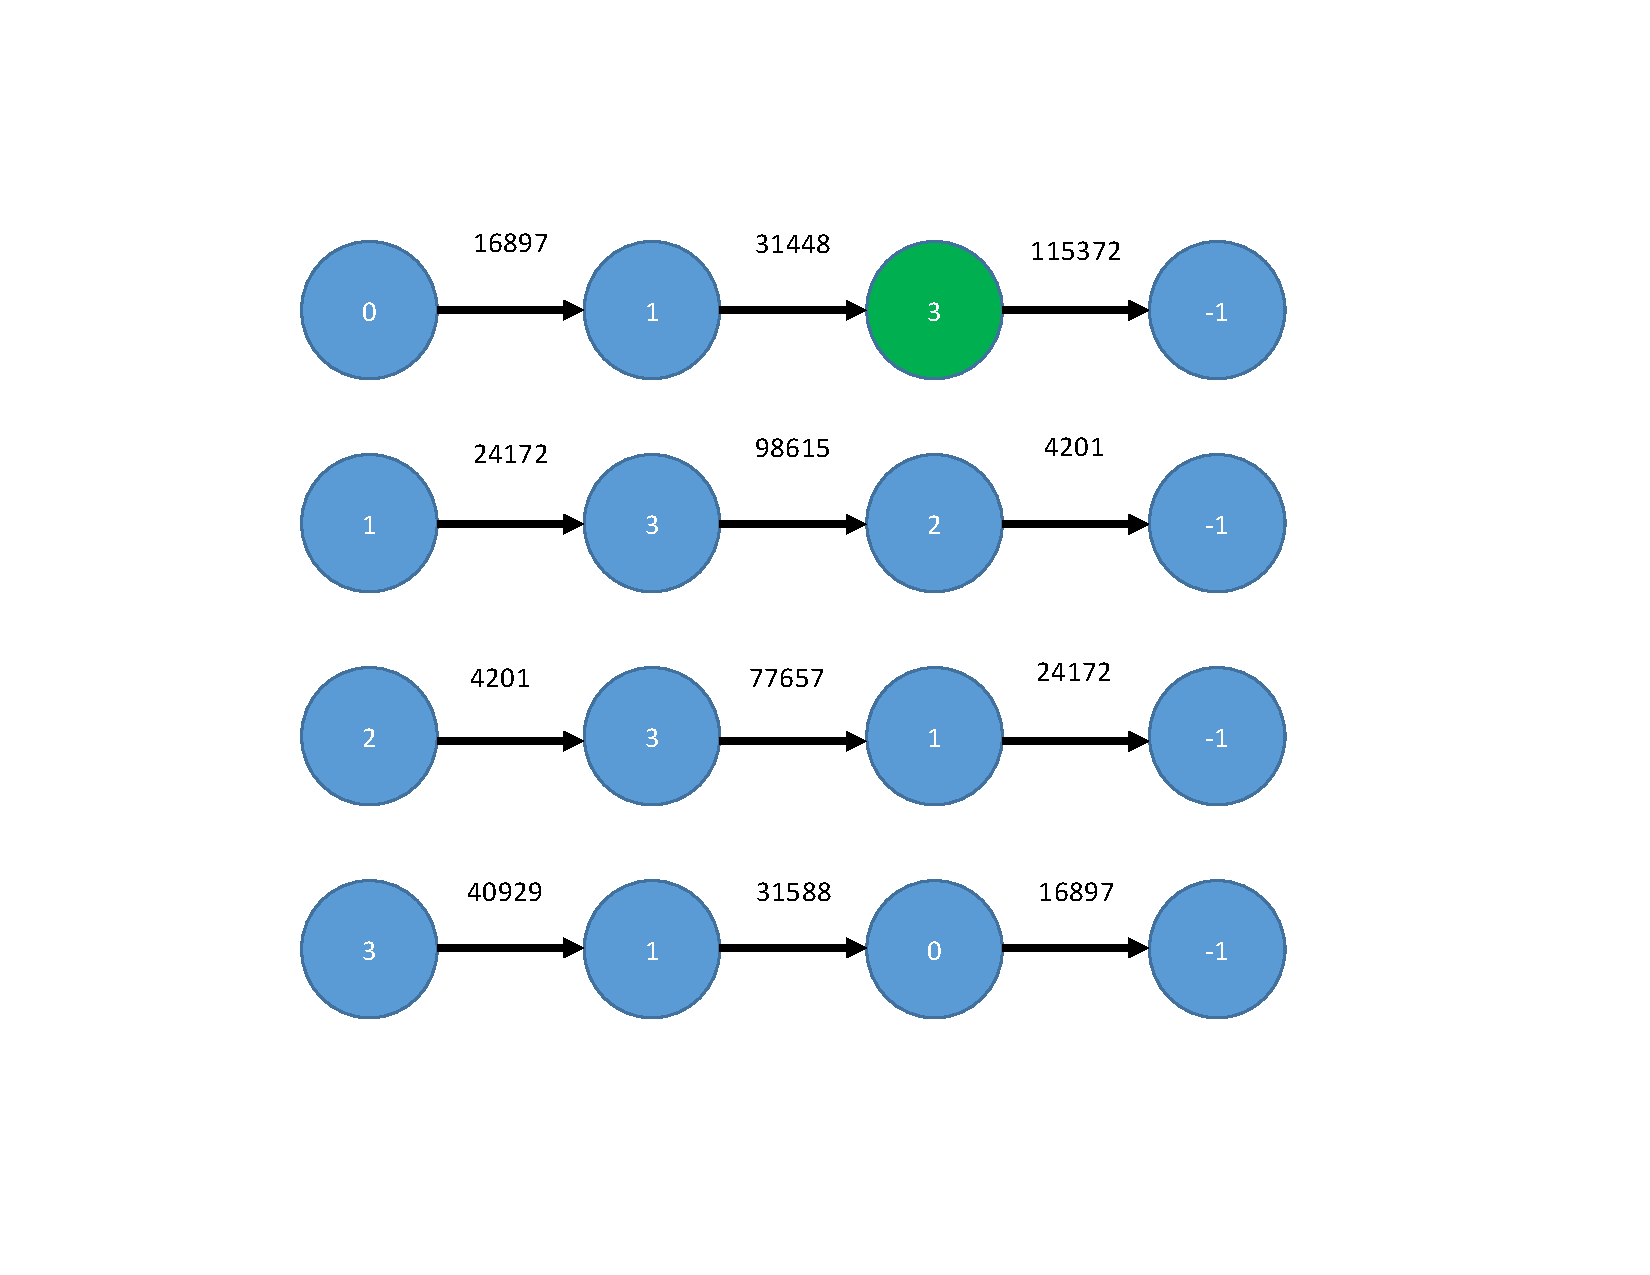
\includegraphics[trim={2cm 2cm 4cm 2cm},clip,scale=0.45]{figures/final.pdf}
\end{frame}

\begin{frame}[t]\frametitle{Current Setbacks}
\begin{block}{}
\begin{itemize}
	\item For perfectly balanced problems, every simple path is the longest path.
	\item Each octant should finish sweeping in the same amount of time.
	\item Current conflict resolution attempts achieve the correct answer for small problems (4-9 subsets), but as the number of paths grows, the octants sweep times no longer match.
	\item Correctly estimating sweep time for perfectly balanced problems is an immediate priority.
\end{itemize}
\end{block}
\end{frame}

\section{Future Work}

\begin{frame}[t]\frametitle{Immediate Priorities}
\begin{block}{}
\begin{itemize}
	\item Correctly estimate sweep time for perfectly balanced partitions.
	\item Add options for angular and spatial aggregation.
	\item Match PDT's results for scaling on perfectly balanced partitions.
\end{itemize}
\end{block}
\end{frame}

\begin{frame}[t]\frametitle{Goals of the Dissertation}
\begin{block}{}
\begin{itemize}
	\item Verify time-to-solution estimator matches PDT's sweep time with equivalent aggregation parameters and scheduling.
	\item Use time-to-solution estimator to optimize cut line locations by using it as a cost function in a Python optimization library (scipy.minimize, scipy.optimize, etc.). 
	\item Build test problems, in 2D and 3D, that balance approximately perfectly via both load balancing algorithms.
	\item Using these test problems, show that optimizing partitions with the proposed approach yields a better runtime.
	\item Implement these tests in PDT and show that the optimized partitions yield a better runtime than perfectly load balanced problems.
	\item Explore adding the threads per processor as a variable to our parameter space during optimization in addition to cut lines.
\end{itemize}
\end{block}
\end{frame}

\end{document}
